\chapter{Axions}\label{chapter:axions}
\lhead{\emph{Axions}}

\section{Introduction}\label{sec:axions_intro}
Because the true identity of dark matter remains unknown it is best that we are open-minded about the types of particle we might hope to detect. In this final Chapter we explore what is probably the second most popular class of dark matter candidate. The axion is an attractive solution, given that it can explain two outstanding problems in physics simultaneously. But nature need not be so generous, hence the generalisation of axions to axion-{\it like} particles (ALPs), is also the subject of some discussion. Although the experimental strategies for detecting axions and ALPs are most of the time very different from WIMPs, many of the issues we have raised in previous Chapters are shared. Whether detecting axions or WIMPs, we must still try to understand the structure of our local dark matter halo.

Terrestrial searches for dark matter axions or ALPs are typically based on their coupling to electromagnetism. In this Chapter we follow analogous strategies to those introduced previously, but we apply them now to microwave cavity haloscope experiments. We simulate signals in a hypothetical future experiment based on ADMX~\cite{Asztalos:2009yp} that could be performed once the axion has been detected and a frequency range containing the axion mass has been identified. We develop a statistical analysis to extract astrophysical parameters and study tidal streams as before. We are now also able to consider classes of substructure particular to axionic dark matter. The example we use here are miniclusters, a prediction of some early Universe axion production mechanisms~\cite{Hogan:1988mp}. One of the goals of this Chapter is to emphasise the differences between measuring a dark matter halo made of axions compared with one made of WIMPs. As we showed in Chapter~\ref{chapter:directional}, even with an angular distribution of WIMP recoils, reconstructing and measuring properties of the local velocity distribution is difficult even with a large number of events. With the detection of axions however, because we observe simply their conversion into photons - rather than via any stochastic scattering process - the prospects are much better. The results we present here point towards the idea that in a post axion discovery era, haloscope experiments may be able to perform ``axion astronomy''.

We begin by outlining the theoretical motivation for dark matter in the form of axions as well as summarising the existing constraints on their existence from experiments, astrophysics and cosmology. We then study the detection of dark matter axions and ALPs with microwave cavity haloscopes. In Sec.~\ref{sec:axions_background} we describe the construction of a haloscope simulation and the development of a statistical analysis that we can use to extract information about the local dark matter halo. We then apply this technique in Sec.~\ref{sec:axions_astronomy}. We first attempt to reconstruct basic input parameters before extending to N-body data from the Via Lactea II (VL2)~\cite{Diemand:2007qr} simulation. Finally, we present a schematic discussion of the detectability of tidal streams from disrupted axion miniclusters. We summarise this Chapter in Sec.~\ref{sec:axions_summary}. 

\section{Background}
\subsection{QCD axions}\label{sec:axions_qcdaxion}
QCD is a relativistic and quantised field theory with invariance under local transformations from SU(3) (the group of unitary matrices of dimension 3). The dimensions of SU(3) lead to the conservation of three colour charges possessed by the quarks, and its eight generators are the gauge bosons known as gluons. The QCD Lagrangian for one generation of massless quarks with left and right handed chiralities, ($u_L,\, u_R,\, d_L,\, d_R)$, is written
\begin{equation}
\mathcal{L}_{\rm QCD} = \sum_{i = u_L,\,u_R,\,d_L,\,d_R} \bar{q}_i i \gamma^{\mu}\mathcal{D}_\mu q_i - \frac{1}{4}G_{\mu \nu}^a G^{\mu \nu}_a \, ,
\end{equation}
where $G^a_{\mu\nu}$ are the gluon field strength tensors. When examining the symmetries of this Lagrangian permitted by the model observables one finds that an axial U(1)$_A$ symmetry that transforms quark chiralities inversely is obeyed. The symmetry should be spontaneously broken though by quark condensates, subsequently giving rise to a boson with a mass slightly larger than the pion. However no such boson is observed. The lack of this particle as well as the discrepancies caused by the breaking of this symmetry on predictions of well studied particle decays led the issue to be known in the 1970s as the U(1)$_A$ problem~\cite{Weinberg:1975ui}. The problem was resolved in this form after the true structure of the QCD vacuum was discovered. In fact the SU(3) gauge fields have an infinite number of vacuum states connected by instanton solutions which cause the QCD vacuum to break the $U(1)_A$ symmetry explicitly thus solving the problem. Though in its place emerged a different one. The density of instanton solutions, parameterised by a phase $\theta$ effectively adds another term to the Lagrangian~\cite{tHooft:1976rip},
\begin{equation}\label{eq:instanton}
\mathcal{L}_{\rm QCD} = ... + \theta \frac{g_s^2}{32 \pi} G^{\mu \nu a} \tilde{G}_{\mu \nu}^a \, ,
\end{equation}
where $g_s$ is the strong coupling constant. This term conserves charge conjugation C, but violates parity P and time reversal T, giving rise to CP-violation in baryons. Additionally, the parameter $\theta$ should be measurable in the form
\begin{equation}
\bar{\theta} = \theta + \arg \det \mathcal{M}_q \ ,
\end{equation}
where $\mathcal{M}_q$ is the quark mass matrix. The appearance of the phase of $\mathcal{M}_q$ is due to the inclusion of CP-violating weak interactions which in general make quark masses complex. Note that the physical parameter $\bar{\theta}$ is the combination of purely weak sector physics, $\arg \det \mathcal{M}_q$, and purely strong sector, $\theta$. Furthermore, this observable can be tightly constrained in experiments which attempt to measure the electric dipole moment (edm) of the neutron. No edm has been observed, meaning that QCD appears to require the fine tuning of $\bar{\theta}$ to a value smaller than $10^{-14}$~\cite{Baker:2006ts}. The essence of the problem is why do two numbers, $\theta$ and $\arg \det \mathcal{M}_q$, so precisely cancel? Both are phases that could take in principle any value from 0 to $2 \pi$, and both have entirely different physical origins. This unnatural absence of CP-violation in QCD is known as the strong CP problem.

A popular and well motivated solution to the strong CP problem devised by Peccei and Quinn~\cite{Peccei:1977hh, Kim:2008hd} (PQ) is to promote the CP-violating phase to a field. The apparent fine tuning of $\theta$ is explained as a dynamical phenomenon: it is driven to 0 because of the spontaneous breaking of a new U(1)$_{\rm PQ}$ symmetry. This new symmetry, and its breaking, is based on a modification of the Higgs mechanism which provides masses to the quarks through Yukawa interactions between them and the non-zero vev of the Higgs field. In this case, the instanton term of Eq.~(\ref{eq:instanton}) tips the Higgs potential to a particular value that depends on $\theta$ which is then picked up in the masses of the quarks. The result is that $\arg \det \mathcal{M}_q$ is set to $-\theta$ and thus $\bar{\theta}$ is driven to 0. The spontaneous breaking of this new U(1)$_{\rm PQ}$ symmetry at some scale $f_a$ produces a new pseudo Nambu-Goldstone boson, dubbed the axion~\cite{Wilczek:1977pj,Weinberg:1977ma}. The axion is given a small mass through instantons which mix it with another neutral boson, the pion. This small mass in terms of the PQ symmetry breaking scale is~\cite{Cheng:1987gp}
\begin{equation}
 m_a = \frac{z^{1/2} f_\pi m_\pi}{f_a(1+z)} \sim 6\,{\rm eV}\left(\frac{10^6\,\,{\rm GeV}}{f_a}\right) \, ,
\end{equation}
where $f_\pi = 92$ MeV is the pion decay constant and $z = m_u/m_d$ is the ratio of the up and down quark masses\footnote{This formula uses the standard value $z=0.56$~\cite{Leutwyler:1996qg} although uncertainty in the quark masses could give values $z = 0.38 - 0.58$~\cite{Agashe:2014kda}.}. Although the original Peccei-Quinn-Weinberg-Wilczek (PQWW) axion, which assumes $f_a$ is around the weak scale, was swiftly ruled out~\cite{Antreasyan:1990cf}, new mechanisms such as those of Kim-Shifman-Vainshtein-Zakharov (KSVZ)~\cite{Kim:1979if,Shifman:1979nz} and Dine-Fischler-Srednicki-Zhitnitsky (DFSZ)~\cite{Dine:1981rt,Zhitnitsky:1980tq} were subsequently constructed. These `invisible' axion models had very small couplings to the standard model making them consistent with known particle data and possible dark matter candidates.

In principle axions are detectable. Initially suggested by Sikivie~\cite{Sikivie:1983ip}, a good way one might hope to see axions in experiments or through astrophysical observation is via their coupling to electromagnetism. One expects axions to be allowed to convert into photons inside magnetic fields in a process known as the Primakoff effect~\cite{Pirmakoff:1951pj}. The interaction is described by a term in the Lagrangian
\begin{equation}\label{eq:interationlagrangian}
 \mathcal{L}_{a\gamma\gamma} = \frac{1}{4} g_{a\gamma\gamma}\, a F_{\mu \nu}\tilde{F}^{\mu \nu} \, ,
\end{equation}
where $F_{\mu \nu}$ is the electromagnetic field strength tensor. For the QCD axion, the axion to two photon coupling, $g_{a\gamma\gamma}$, has a fixed relationship with the decay constant, $f_a$ (and in turn $m_a$), given by the formula
\begin{equation}\label{eq:qcdcoupling}
 g_{a\gamma\gamma} = \frac{g_\gamma \alpha}{\pi f_a} \, ,
\end{equation}
where $\alpha$ is the fine structure constant. The dimensionless coupling $g_\gamma$ is,
\begin{equation}
 g_\gamma = \frac{1}{2}\left(\frac{E}{N} - \frac{2}{3}\frac{4+z}{1+z}\right) \, .
\end{equation}
In which  $E/N$ is the ratio of the colour axion anomaly to the electromagnetic axion anomaly. The value of this constant is model dependent: $E/N=-0.97$ for the KSVZ model and $0.36$ for the DFSZ model for example.

\subsection{Axion-like particles}\label{sec:axions_alps}
The PQ-mechanism functions independently of the scale of $m_a$, meaning that in the absence of any preference, searches for the axion should need to take place over many orders of magnitude. Worse still, the well defined relationship between $g_{a\gamma\gamma}$ and $f_a$ of Eq.~(\ref{eq:qcdcoupling}) means that for much of the mass range, measuring the corresponding coupling would require incredibly sensitive experiments. Instead, when describing techniques designed to search for $g_{a\gamma\gamma}$, the picture is generalised to include any light pseudoscalar particle that couples in the same manner. This unveils a wider parameter space of axion-like particles that are not restrained by the relationship between $m_a$ and $f_a$. Axion-like particles include any other pseudo Nambu-Goldstone bosons that are associated with the breaking of global symmetries, but not necessarily the Peccei-Quinn symmetry.

When placing constraints on $m_a$ and $g_{a\gamma\gamma}$ it is standard practice to remain agnostic with regards to the origin of the ALP and approach searches purely phenomenologically, i.e. by simply constraining interactions with the of form Eq.~(\ref{eq:interationlagrangian}). It has been shown however that such particles appear frequently in the low energy spectrum of many standard model extensions. The most notable of these is the generic prediction of many axion-like particles (in addition to the QCD axion~\cite{Cicoli:2012sz}) in models of string theory~\cite{Svrcek:2006yi}. This so-called `axiverse' of ALPs may be exhibited over a huge range of mass scales, down to the `ultralight' regime set by the Hubble scale $\sim10^{-33}$~eV~\cite{Arvanitaki:2009fg}. Additionally in some models of SUSY breaking which require a spontaneously broken R-symmetry, the subsequent pseudo-Nambu Goldstone boson may also appear in searches for ALPs~\cite{Nelson:1993nf}. Similar classes of particle produced by the breaking of, for example, family symmetries~\cite{Jaeckel:2013uva} or lepton number~\cite{Chikashige:1980ui} have also been demonstrated to couple in the manner of an axion.

The generalisation to ALPs is further motivated by an assortment of astrophysical hints for the existence of a non-QCD axion. Several excesses and irregularities in X-ray~\cite{Bulbul:2014sua,Boyarsky:2014jta,Berg:2016ese} emission in various sources, for example, could be explained by decaying or interacting ALPs~\cite{Conlon:2013txa,Conlon:2014wna}. Observations of TeV $\gamma$-rays also seem to suggest the Universe is anomalously transparent even when propagation at those energies should be suppressed by electron pair production with the extragalactic background light~\cite{Aharonian:2005gh,Mazin:2007pn,Aliu:2008ay,Ackermann:2012sza,Abramowski:2012ry}. One explanation for this transparency invokes axion-photon conversion over astronomical distances allowing $\gamma$-rays to travel further than usual~\cite{DeAngelis:2011id,Wang:2015dil}. A range of measurements of  white dwarfs~\cite{Isern:2008nt}\footnote{Of these hints, currently only the white dwarf cooling hint can be explained by a QCD axion.}, red giants~\cite{Viaux:2013lha}, horizontal branch~\cite{Ayala:2014pea}, and neutron stars~\cite{Leinson:2014ioa}, have occasionally been better explained if ALPs are provided as an additional heat loss mechanism. As is often the case with indirect dark matter claims, the sources of systematic uncertainty are plentiful and they may all have astrophysical explanations.

\subsection{Axions and ALPs as dark matter}\label{sec:axions_axionsdm}
ALPs, and the QCD axion in particular, would be attractive candidates for dark matter, but it must be demonstrated first that such light bosonic particles can be produced in the correct abundance and have phenomenology that matches the known properties of CDM. For instance, because QCD axion couplings scale inversely with its mass, we can immediately dismiss axions heavy enough to thermalise in the early Universe while still relativistic; existing today as a hot dark matter contribution to the energy density of the Universe. As discussed in Chapter~\ref{chapter:intro}, hot dark matter cosmologies are strongly disfavoured due to the suppression of structure formation on small scales. Moreover, additional relativistic species modify the damping tail of the CMB and also affect the abundances of the primordial elements produced during nucleosynthesis. For these reasons there is an upper bound of $m_a < 0.529$~eV on the QCD axion as HDM from a combination of Planck temperature, polarisation and SZ cluster count data, as well as expansion rate and matter power spectrum measurements from other cosmological datasets~\cite{DiValentino:2015wba}. Thermally produced ALPs on the other hand are still allowed as a dark matter candidate for some ranges of mass and coupling~\cite{Cadamuro:2010cz}.

For smaller masses, axions can be produced efficiently by alternative non-thermal mechanisms. A well known example is the vacuum misalignment mechanism in which axions are produced by oscillations in the field as it relaxes into the minimum of its potential shortly after the symmetry breaking phase transition~\cite{Abbott:1982af,Dine:1982ah,Preskill:1982cy}. The equation of motion for the CP violating phase $\bar{\theta}$ can be approximated by taking a mass term for the axion potential, the dynamics will follow that of a simple harmonic oscillator with a damping term provided by Hubble expansion $H(t)$,
\begin{equation}
 \ddot{\bar{\theta}} + 3 H(t) \dot{\bar{\theta}} + m_a^2\bar{\theta} = 0\, .
\end{equation}
The rms value of the $\bar{\theta}$ field at some time sets the abundance of particles. Hence the number of axions produced through this mechanism depends on the axion mass and the initial misalignment angle $\bar{\theta}_0$ that dictates how long oscillations persist~\cite{Marsh:2015xka},
\begin{equation}
 \Omega_a h^2 \simeq 0.4 \, \left(\frac{6\,\mu{\rm eV}}{m_a}\right)^{7/6} \langle \bar{\theta}_0^2\rangle \, .
\end{equation}
This relationship implies that for small masses, small values of the initial misalignment angle are needed to avoid producing too much dark matter. Heavier axions on the other hand can still be produced in the right amounts providing $\bar{\theta}_0$ is tuned very close $\pi$; in this regime anharmonic corrections to the harmonic potential end up boosting the production of axions~\cite{Visinelli:2009zm}. These two conditions must be balanced if one assumes that the PQ symmetry breaking has already occurred before inflation~\cite{Preskill:1982cy,Abbott:1982af,Dine:1982ah}. In this scenario a single causal patch containing some random value of $\langle \bar{\theta}_0^2\rangle$ gets inflated to the horizon size so we could have any value in our observable Universe.

The situation is slightly different however if inflation occurs {\it before} the PQ symmetry breaking phase transition. In this case the balancing of masses and tuning of misalignment angles is not needed since $\bar{\theta}$ should be a randomly distributed field for which $\langle \bar{\theta}_0^2\rangle = \pi^2/3$. Ensuring the density of axions produced via this mechanism doesn't exceed the density of dark matter (as well as satisfying astrophysical constraints, see Sec.~\ref{sec:axions_constraints}) leads to the ``classic'' axion window $m_a \sim 80~-400\,\mu$eV~\cite{Hiramatsu:2012gg}. There are large uncertainties on the natural range of masses however because the abundance calculation is complicated further by the presence of topological defects produced at the phase transition. These are not a concern if the PQ symmetry is broken before inflation because the defects are simply inflated away. But here the additional population of axions produced from the decay of axion strings and domain walls, as well as the cosmological implications of such defects must be considered. For example, domain walls occurring in the DFSZ model are particularly problematic as they quickly dominate the energy density and are completely incompatible with the present day Universe. Cosmic axion strings may also seed clumps of axions known as miniclusters~\cite{Hogan:1988mp,Kolb:1993zz,Kolb:1993hw,Kolb:1994fi,Kolb:1995bu,Berezinsky:2013fxa,Tinyakov:2015cgg,Fairbairn:2017dmf}, the observational prospects of which we discuss later in this Chapter.

To be dark matter though, axions must not only be produced with the correct cosmological abundance they must also behave like CDM and form structure in agreement with our own Universe. Because axions will have their interactions suppressed by $f_a$, they will almost certainly be weakly coupled enough to appear stable on cosmological timescales. It will also mean that axions produced via non-thermal mechanisms will behave like cold and collisionless particles so naturally recover a matter power spectrum that extends over scales matching the observed sizes of halos and subhalos in our Universe. Interestingly, ultralight axions ($m_a \approx 10^{-21}$~eV) in particular may improve upon CDM, and have been suggested as a solution to problems with the overabundance of small scale structure in simulations~\cite{Marsh:2015wka,Hu:2000ke,Marsh:2013ywa}.

Notably in the literature there has been an ongoing discussion about the formation of Bose-Einstein condensates (BECs) of axions with huge occupation numbers and cosmologically sized correlation lengths. This idea was initially motivated by attempts to find properties of axionic dark matter that in some way distinguished them from WIMPs. It was suggested by Sikivie that a halo constructed from a condensate of axions could form vortices leading to observable ring-like caustics~\cite{Sikivie:2009qn,Erken:2011dz}. It was then subsequently countered that the axion self-interactions in fact had the wrong sign to allow vortices to form~\cite{RindlerDaller:2011kx}. The issue is still under debate, largely centered around if a BEC formed from a cosmological population of axions~\cite{Davidson:2014hfa}, and the role of gravity and axionic self-interactions in sustaining it if so~\cite{Guth:2014hsa,Davidson:2013aba}.
 

\subsection{Constraints on axions}\label{sec:axions_constraints}
\begin{figure}
\begin{center}
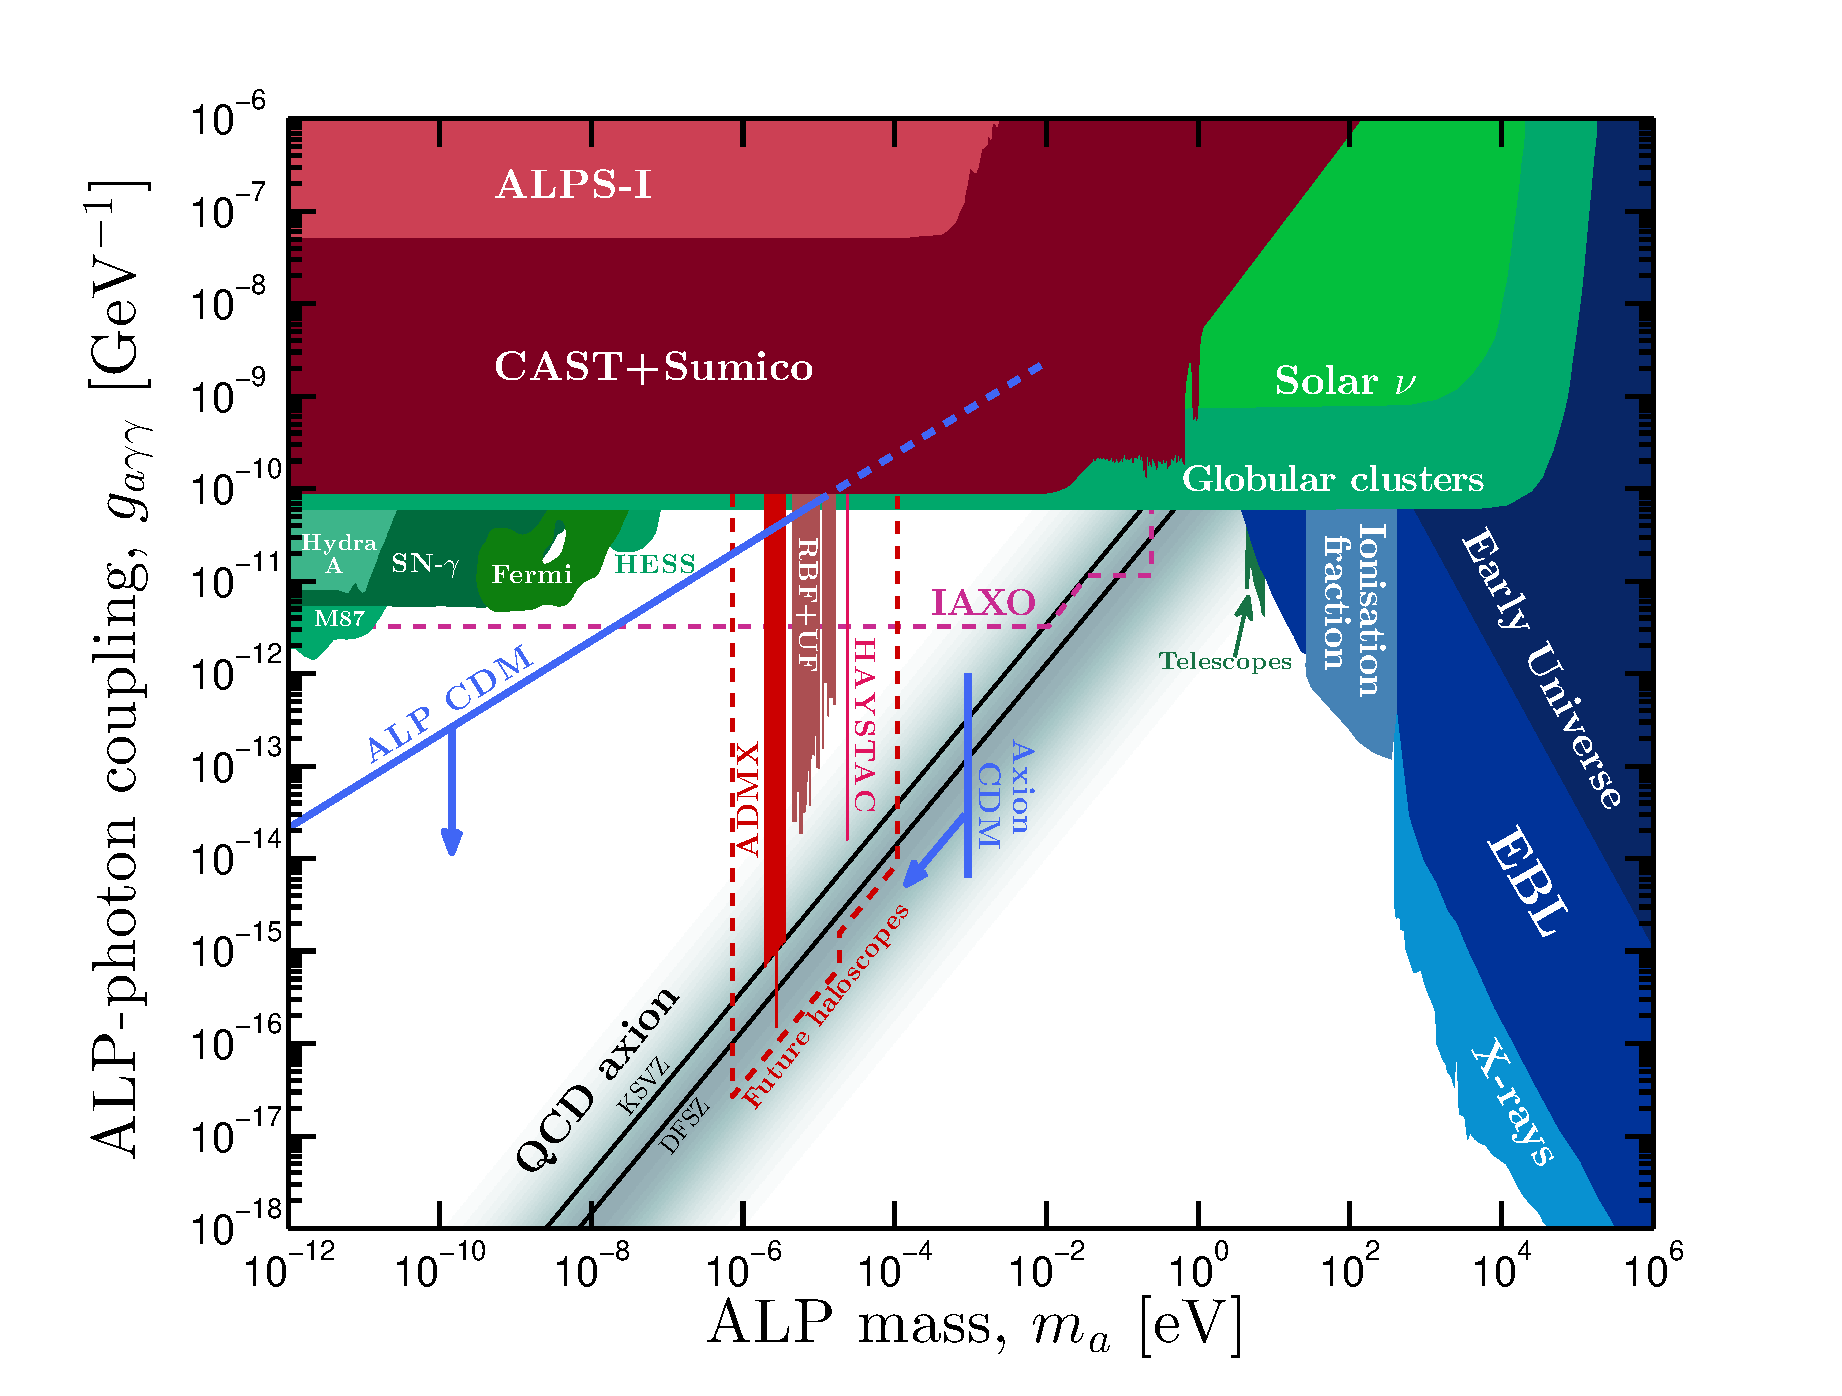
\includegraphics[width=\textwidth]{Figures/axionconstraints.eps}
\caption[Constraints on the ALP-photon coupling]{Constraints on the axion-photon coupling $g_{a\gamma\gamma}$ as a function of axion/ALP mass $m_a$. Experimental bounds are filled in various shades of red, astrophysical constraints in shades of green, and bounds from cosmology are in shades of blue. An explanation for each constraint is given in the text. We also indicate a band showing the relationship between the coupling and mass for the QCD axion; the KSVZ and DFSZ models are shown as black lines.}\label{fig:axionconstraints}
\end{center}
\end{figure}
Here, we summarise the status of experimental and observational searches based on the Primakoff conversion between axions/ALPs and photons\footnote{We do not discuss them at length here but many constraints on axions/ALPs can be applied to dark photons (sometimes called hidden photons) which could arise from additional U(1)s added to the standard model gauge group that are obeyed by some dark sector~\cite{Holdom:1985ag}. This allows for kinetic mixing terms which convert photons to dark photons and vice versa, in a similar way to ALPs. For a review see, e.g. Ref.~\cite{Jaeckel:2013ija}.}. We show existing constraints on the $m_a - g_{a\gamma\gamma}$ plane in Fig.~\ref{fig:axionconstraints}, we also indicate the projected reach of some future experiments. We describe each constraint below.

{\color{Red}{\bf Experimental searches}} (red in Fig.~\ref{fig:axionconstraints})\vspace{-1em}
\begin{itemize} \itemsep0em 
 \item {\bf Haloscopes} are resonant cavity experiments searching for photons from dark matter axions converting inside the magnetic field. The photon power is enhanced when the mode frequency equals $m_a$. The mass range accessible to a haloscope is controlled range of frequencies over which the resonance of the cavity can be tuned. The smallest accessible coupling on the other hand is controlled by the signal-to-noise level. The most sensitive resonant cavity experiment, ADMX, has constrained masses in microwave frequencies, $1.9\,\mu{\rm eV} < m_a < 3.69\,\mu{\rm eV}$~\cite{Asztalos:2009yp,Hoskins:2011iv} and has reached QCD axion models. We also show the most recent limit from the first results of the prototype Yale Wright Laboratory experiment~\cite{Brubaker:2016ktl}, currently only constraining in a very small range $m_a\sim 20\,\mu$eV. Earlier haloscopes such as the Rochester-Brookhaven-Fermilab (RBF)~\cite{DePanfilis:1987dk} and University of Florida (UF)~\cite{Hagmann:1990tj} experiments have also probed slightly larger masses but with lower sensitivity.
 \item {\bf Helioscopes}: The CAST~\cite{Zioutas:2004hi} and Sumico experiments~\cite{Inoue:2002qy} search for Solar axions and ALPs. These are produced in the large electromagnetic fields in the plasma of the Sun so rely on well studied Solar physics~\cite{Redondo:2013wwa}. The flux of axions is predicted with energies in the keV range and will Primakoff convert into X-rays inside magnetic cavities. For light ALPs with kinetic energy much higher than their mass the conversion probability is coherent up to around $\mathcal{O}(10^{-2})$~eV meaning a swath of masses below this can be ruled out based on the non-observation of the expected Solar axion conversion peak. Up to slightly larger masses, $m_a\sim$~eV, the sensitivity of a helioscope can be extended with the injection of a buffer gas, such as $^3$He or $^4$He, that restores the coherence effect. The pressure of the gas is slowly adjusted, refracting the photons to a range of effective masses corresponding to a range of $m_a$~\cite{vanBibber:1988ge}.
 \item {\bf Light-shining-through-a-wall (LSW) experiments} are purely laboratory based and look for the conversion of photons from a laser beam passing through a strong magnetic field into ALPs on either side of an opaque boundary. The ALPS-I~\cite{Bahre:2013ywa} experiment is sensitive to a wide range of light masses. The signal in LSW experiments is unfortunately suppressed by an extra factor of $g_{a\gamma\gamma}^2$ compared with haloscopes and helioscopes because it relies on {\it two} instances of axion-photon conversion. The ALPS experiment currently lacks the sensitivity to reach the QCD axion.
 \item {\bf Future experiments}: We indicate the reach of future experiments that are either planned or have been proposed. These include the planned next generation helioscope IAXO~\cite{Armengaud:2014gea} and a range of alternative haloscopes designed to probe beyond the technological restrictions of ADMX: ADMX-HF~\cite{Simanovskaia:2015fdi}, QUAX~\cite{Ruoso:2015ytk}, MADMAX~\cite{TheMADMAXWorkingGroup:2016hpc} and CULTASK~\cite{Chung:2016ysi}.
\end{itemize}

{\color{Green}{\bf Astrophysical bounds}} (green in Fig.~\ref{fig:axionconstraints})\vspace{-1em}
\begin{itemize}\itemsep0em 
 \item {\bf Globular clusters}: Stars that are in the ``horizontal branch'' of a globular cluster colour-magnitude diagram have entered their helium burning phase. The number of stars observed in this region relative to the total number of red giant stars is then a good estimate of the length of time spent burning helium. Since ALP production would accelerate this phase of a star's life, counts of horizontal branch stars in globular cluster observations place stringent limits on $g_{a\gamma\gamma}$~\cite{Ayala:2014pea}.
 \item {\bf Solar $\boldsymbol{\nu}$}: Axion production in the Sun would lead to an increased nuclear fusion rate and a hotter interior. The highly temperature dependent flux of $^8$B neutrinos is then a good probe of energy loss via axion production~\cite{Gondolo:2008dd}. Comparisons of axion-modified Solar models with neutrino data place constraints on $g_{a\gamma\gamma}$ for axion masses less than the core temperature of the Sun~\cite{Vinyoles:2015aba}.
 \item {\bf Supernovae}: If produced in SN, ALPs would be expected to Primakoff convert into $\gamma$-rays in the magnetic field of the Milky Way. The non-observation of $\gamma$-rays coincident with neutrinos from the 1987 supernova in the Large Magellanic Cloud (SN1987A) excludes a region of ultralight ALPs with $m_a \lesssim 4.4 \times 10^{-10}$~eV and $g_{a\gamma\gamma} \lesssim 5.3 \times 10^{-12}$~GeV$^{-1}$~\cite{Payez:2014xsa}. Additionally, though we do not show these in Fig.~\ref{fig:axionconstraints}, the neutrino burst duration~\cite{Raffelt:2006cw} and the absence of photons from heavier {\it decaying} axions~\cite{Jaeckel:2017tud} (also in SN1987A) exclude regions overlapping with cosmological constraints (described below). As pointed out by Ref.~\cite{Jaeckel:2017tud}, if another nearby Supernova occurs at some point in the near future we can expect limits of this type to dramatically improve.
 \item {\bf Fermi}: Photon-ALP mixing is expected to be imprinted on $\gamma$-ray spectra for $m_a\lesssim\mu$eV in a way that depends on the structure of the magnetic field through which they pass. A search for such irregularities in NGC 1275 by Fermi-LAT has constrained $g_{a\gamma\gamma}\lesssim 5\times10^{-12}$~GeV$^{-1}$~\cite{TheFermi-LAT:2016zue}.
 \item {\bf Hydra-A}: Similar constraints have been made using Chandra observations of a bright X-ray source at the centre of the Hydra cluster~\cite{Wouters:2013hua}.
 \item {\bf HESS}: The bright blazar PKS 2155-304 would also be expected to show $\gamma$-ray irregularities, the lack of which as seen by HESS has set to constraints on masses around $10^{-8}$~eV~\cite{Wouters:2013iya}.
\item {\bf M87}: Recent analysis of Chandra observations of the radio galaxy M87 in the Virgo cluster by Ref.~\cite{Marsh:2017yvc} also find an absence of any irregularities.
\end{itemize}

{\color{Blue}{\bf Cosmological bounds}} (blue in Fig.~\ref{fig:axionconstraints})
We indicate with two lines the regions of the parameter space for which axions or ALPs can roughly constitute the cosmological population of CDM~\cite{Essig:2013lka}. Cosmological data can also be used to rule out mass and coupling regions,\vspace{-1em}
\begin{itemize}\itemsep0em 
 \item{ \bf Ionisation fraction}: The recombination of hydrogen atoms freezes out at $z\sim800$ leaving a residual fraction, $x_{\rm ion}$, of primordial matter ionised until the Universe becomes reionised at some point between $z\sim6-15$~\cite{Zaroubi:2012in}. This residual fraction can be inferred from measurements of the optical depth with CMB data. Before reionisation there could not have been any large quantity of excess ionisation due to UV photons from, for instance, decaying ALPs with masses $m_a \sim 13.6 - 300$ eV (the energy levels of hydrogen)~\cite{Arias:2012az,Cadamuro:2012rm}.
 \item {\bf Extragalactic background light (EBL)}: The decay of ALPs over the age of the Universe would lead to a redshift broadened peak in diffuse background emission at energies set by half the axion mass. No such peak is observed in the EBL which extends from microwave to $\gamma$ wavelengths~\cite{Overduin:2004sz}. 
 \item {\bf Telescopes}: By similar arguments ALPs can be constrained in the visible spectrum with optical telescopes by searching for their decay in the spectra of galaxy clusters~\cite{Grin:2006aw}.
 \item {\bf X-rays}: ALP masses up to X-ray energies can be constrained to very small couplings thanks to sensitive searches for lines in observations by Chandra, XMM-Newton, INTEGRAL and Suzaku (this region has been translated from the equivalent bounds on decaying sterile neutrinos)~\cite{Boyarsky:2009ix}.
 \item {\bf Early Universe}: If axions decay into photons before recombination then they must do so infrequently enough to not cause any major spectral distortions to the CMB, contribute to the number of effective species of neutrino beyond the current estimates, or alter the abundances of primordial elements in contradiction to BBN~\cite{Cadamuro:2012rm}.
\end{itemize}

We emphasise again that out of the several experimental searches for axions, {\it only} haloscopes can test them as a dark matter candidate. Some astrophysical and cosmological constraints, for example X-ray and optical telescope searches, assume ALP dark matter halos, but the majority are centered around their production or decay. We now wish to determine how the local dark matter distribution can be measured if axions or ALPs are dark matter instead of WIMPs, so we must consider haloscopes.


\section{Simulating a haloscope experiment}\label{sec:axions_background}

\subsection{Axions in a magnetic field}\label{sec:axions_theory}
We begin by outlining some of the essential steps in calculating the resonantly enhanced axion-photon conversion power inside a magnetic cavity. Full details of these calculations can be found in Refs.~\cite{Hong:2014vua,McAllister:2015zcz,Krauss:1985ub}. We follow the conventions adopted in Ref.~\cite{Hong:2014vua} but now that we wish to make the connection to realistic halo velocity distributions, we depart from an often used approximation that the axion power spectrum can be described with a Breit-Wigner function\footnote{After the completion of this work a new study of astrophysically motivated signal models for axion searches was presented in Ref.~\cite{Lentz:2017aay}. These models also depart from a Breit-Wigner approximation.}.

The effective Lagrangian for axions coupled to electromagnetism is
\begin{equation}
 \mathcal{L} = \frac{1}{2}\partial_\mu a \partial^\mu a - V(a) + \frac{1}{4}g_{a\gamma\gamma} a F_{\mu\nu}\tilde{F}^{\mu\nu}
    - \frac{1}{4}F_{\mu\nu}F^{\mu\nu} + j^\mu A_\mu + a\rho_q \, ,
\end{equation}
where $F_{\mu\nu}$ is the electromagnetic field strength tensor and $\tilde{F}^{\mu\nu}~=~\frac{1}{2}\epsilon^{\mu\nu\rho\sigma}F_{\rho\sigma}$ its dual. The axion potential $V(a)$ is provided by QCD instanton effects and can be approximated with a simple mass term $\frac{1}{2} m_a^2 a^2$. The axionic charge density and the electromagnetic current density are written as $\rho_q$ and $j^\mu$. Writing $F_{\mu\nu}\tilde{F}^{\mu\nu}~=~-~4\,\textbf{E}\cdot\textbf{B}$ we then see the axion-photon interaction in terms of electric and magnetic field strengths is
\begin{equation}
 \mathcal{L}_{a\gamma\gamma} = - g_{a\gamma\gamma}\, a \textbf{E}\cdot\textbf{B} \, .
\end{equation}
This interaction modifies Maxwell's equations to include an additional axion current,
\begin{eqnarray}
&\nabla \cdot \textbf{E} &= \rho_q + g_{a\gamma\gamma} \nabla a \cdot \textbf{B} \,, \\
&\nabla \cdot \textbf{B} &= 0 \,, \\
&\nabla \times \textbf{E} &= -\frac{\partial \textbf{B}}{\partial t}\,,  \\
&\nabla \times \textbf{B} &= \mu_0\textbf{j} + \frac{\partial \textbf{E}}{\partial t} - g_{a\gamma\gamma} \textbf{B}_0\frac{\partial a}{\partial t} - g_{a\gamma\gamma} \nabla a \times \textbf{E} \, .\quad\quad
\end{eqnarray}
However these equations simplify for the setup we consider here. Firstly we assume the axion field has no spatial dependence on laboratory scales ($\nabla a = 0$). We can do this because the size of ADMX is around the 1~m scale so is well below the de Broglie wavelength of the axion field for the mass ranges we consider ($>$100~m). This allows us to assume that there is no spatial dependence in the axion field over the dimensions of the cavity and hence no additional modulations due to the changing orientation of the cavity with respect to the axion wind. We also assume that there is no axionic charge and no electromagnetic current inside the cavity: $\rho_q = 0$ and $j^\mu = 0$. This results in the following simple set of equations,
\begin{eqnarray}
&\nabla \cdot \textbf{E} &= 0 \,, \\
&\nabla \cdot \textbf{B} &= 0 \,, \\
&\nabla \times \textbf{E} &= -\frac{\partial \textbf{B}}{\partial t} \,, \\
&\nabla \times \textbf{B} &= \frac{\partial \textbf{E}}{\partial t} - g_{a\gamma\gamma} \textbf{B}_0\frac{\partial a}{\partial t} \, .
\end{eqnarray}

Under the above assumptions the equation of motion for the axion field is,
\begin{equation}
 \Box a \simeq \frac{\partial^2 a}{\partial t^2}= -V'(a) - g_{a\gamma\gamma}\textbf{E}\cdot\textbf{B} \, .
\end{equation}

Dark matter axions in the local Milky Way undergo essentially no interactions, so in a quadratic potential $V(a)~\simeq~\frac{1}{2} m_a^2 a^2$, the field oscillates coherently at the axion mass $a(t) = a_0 e^{im_a t} \equiv a_0 e^{i\omega t}$. However this coherence is spoiled slightly by a dispersion in axion velocities: $ \omega = m_a(1+\frac{1}{2}v^2 + \mathcal{O}(v^4))$. One can account for this by moving to a Fourier description of the field, written as $\mathcal{A}(\omega)$,
\begin{eqnarray}
 a(t) &=& \sqrt{T} \int_{-\infty}^{+\infty} \frac{\textrm{d}\omega}{2\pi} \mathcal{A}(\omega) e^{-i\omega t} \,, \\
 \mathcal{A}(\omega) &=& \frac{1}{\sqrt{T}} \int_{-T/2}^{T/2} \textrm{d}t \,  a(t) e^{i\omega t} \, ,
\end{eqnarray}
where $T$ is some large reference time used to take the averages. The quantity $|\mathcal{A}(\omega)|^2$ is referred to as the axion power spectrum. The rms of the axion field squared is connected to the axion power spectrum by the Parseval relation,
\begin{equation}\label{eq:parseval}
 \langle a^2(t) \rangle = \frac{1}{T} \int_{-T/2}^{T/2} \textrm{d} t\, a^2(t) = \int_{-\infty}^{+\infty} \frac{\textrm{d}\omega}{2\pi} |\mathcal{A}(\omega)|^2 \, .
\end{equation} 

The convention we have adopted in previous Chapters for WIMPs is to use a velocity distribution to describe the kinematic structure of the local halo. Now in the context of axions we must relate this somehow to a classically oscillating field. In terms of the power spectrum, The velocity distribution is related in the following way. First we write down the distribution of axion velocities $f_\textrm{lab}(\textbf{v})$ in the laboratory frame by temporarily introducing a number density,
\begin{equation}
 \textrm{d}n = n_0 f_\textrm{lab}(\textbf{v}) \textrm{d}^3 v \, ,
\end{equation}
where $\textrm{d}n$ is the number density of ``particles'' with speeds between $v$ and $v + \textrm{d}v$. The constant $n_0$ is found by integrating $\textrm{d}n$ over all velocities and is used to define the local axion number density $n_0 \equiv \rho_a/m_a$. This allows the connection to be made with a classical field oscillating at $m_a$ which should have $\langle a^2(t)\rangle = n /m_a $,~\cite{Krauss:1985ub}.

An expression for the axion power spectrum $|\mathcal{A}(\omega)|^2$  can be obtained by satisfying Parseval's relation and changing variables from $\omega$ to $v$,
\begin{equation}
|\mathcal{A}(\omega)|^2 = 2\pi \frac{\textrm{d}\langle a^2(t) \rangle}{\textrm{d}v}\frac{\textrm{d}v}{\textrm{d}\omega} \, ,
\end{equation}
we can then substitute for $\textrm{d}\langle a^2(t) \rangle /\textrm{d}v$ using,
\begin{eqnarray}
 \frac{\textrm{d}n}{\textrm{d}v} &=& n_0 \int v^2 f_\textrm{lab}(\textbf{v}) \textrm{d}\Omega \\
  &=& n_0 f_\textrm{lab}(v) \, .
\end{eqnarray}
Hence, the formula for the axion power spectrum on Earth can be written as,
\begin{equation}\label{eq:Asqlab}
|\mathcal{A}(\omega)|^2 = 2\pi \frac{\rho_a}{m_a^2} f_\textrm{lab}(v)\frac{\textrm{d}v}{\textrm{d}\omega} \, ,
\end{equation}
The axion power spectrum is 0 for $\omega<m_a$ which is enforced by requiring that $v$ be real. To avoid confusion with $a(t)$ we have suppressed the time dependence in the velocity distribution here, but we do still expect $|\mathcal{A}(\omega)|$ to modulate annually due to $\textbf{v}_\textrm{lab}(t)$.


\subsection{Resonance power}\label{sec:axions_experiment}
We model a microwave cavity experiment with a static uniform magnetic field $\textbf{B}_0$ maintained inside a cylindrical cavity of radius $R$ and length $L$, with radial, azimuthal and vertical coordinates labelled $(\hat{\textbf{r}},\boldsymbol{\hat{\phi}},\hat{\textbf{z}})$ respectively. The magnetic field is generated by a solenoid with current density in the $\boldsymbol{\hat{\phi}}$-direction. The electric and magnetic fields we write as
\begin{eqnarray}
  \textbf{E}_0 &=& 0 \\
  \textbf{B}_0 &=& n_L I \Theta (R-r)\hat{\textbf{z}} \, ,
\end{eqnarray}
where $\Theta(r)$ is the Heaviside step function, $I$ is the current and $n_L$ is the number of wire turns in the solenoid per unit length. For convenience we use the magnitude of the magnetic field $B_0 = n_L I$ in the following expressions. 

In the cylindrical cavity design the important cavity mode orientations are the TM$_{0l0}$ modes which have transverse magnetic fields in the $\boldsymbol{\hat{\phi}}$-direction (and hence have associated electric fields in the $\hat{\textbf{z}}$-direction). It is useful to write these induced fields in terms of their Fourier components,
\begin{eqnarray}
\textbf{E}_a &=& E^z_a(r,t)\hat{\textbf{z}} =  \left(\sqrt{T} \int_{-\infty}^{+\infty} \frac{\textrm{d} \omega}{2\pi} E_a(r,\omega) \, e^{-i\omega t} \right) \hat{\textbf{z}} \, , \nonumber \\
\textbf{B}_a &=& B^\phi_a (r,t)\hat{\boldsymbol{\phi}} = \left(\sqrt{T} \int_{-\infty}^{+\infty} \frac{\textrm{d} \omega}{2\pi} B_a(r,\omega) \, e^{-i\omega t} \right) \hat{\boldsymbol{\phi}} \, .\nonumber
\end{eqnarray}
In this case, Amp\`{e}re's law from Maxwell's equations reduces to
\begin{equation}
 \nabla \times (\textbf{B}_0 + \textbf{B}_a) = \frac{\partial}{\partial t}(\textbf{E}_0 + \textbf{E}_a) - g_{a\gamma\gamma} (\textbf{B}_0 + \textbf{B}_a) \frac{\partial a}{\partial t} \, .
\end{equation}

Solving this equation inside and outside the cavity and matching boundary conditions leads one to a solution for the Fourier components of the axion generated magnetic and electric fields. The solutions are resonances at particular frequencies corresponding to the zeroes of a Bessel function (although we will only be interested in the lowest resonance which we label $\omega_0$). Following the derivation of Ref.~\cite{Hong:2014vua}, the axion power is calculated by evaluating the following integral over the volume of the cavity $V$,
\begin{equation}
 P = \frac{\omega_0 U}{Q} = \frac{\omega_0}{Q}\int_V \textrm{d}^3 r \Bigg\langle \frac{\textbf{E}_a^2 + \textbf{B}_a^2}{2}\Bigg\rangle \, ,
\end{equation}
where $U$ is the energy stored in the electric and magnetic fields inside the cavity. This expression introduces the quality factor $Q$ which is a number that quantifies how well the cavity stores energy and depends on the material properties of the cavity wall. Evaluating the above formula with the solution for the Fourier components of the axion electric and magnetic fields (which are expressed in terms of $|\mathcal{A}(\omega)|^2$) one arrives at
\begin{equation}\label{eq:axionpower}
 P = g_{a\gamma\gamma}^2 B_0^2 V\omega_0 Q^3 \frac{4}{\chi_{0l}^2} \int_{-\infty}^{+\infty} \frac{\textrm{d}\omega}{2\pi} \mathcal{T}(\omega)|\mathcal{A}(\omega)|^2 \, .
\end{equation}
where $\chi_{0l}$ is the $l$-th zero of the 0th Bessel function of the first kind. We have also defined $\mathcal{T}(\omega)$, which is a Lorentzian that describes the loss in power off resonance,
\begin{equation}
 \mathcal{T}(\omega) = \frac{1}{1+4Q^2\left(\frac{\omega}{\omega_0} - 1\right)^2} \, .
\end{equation}

Usually the haloscope power is written in terms of a cavity form factor, $C_{nlm}$. For the transverse magnetic field\footnote{Other mode orientations, the transverse electric (TE$_{nlm}$) and transverse electromagnetic (TEM$_{nlm}$) modes both have no axial electric field meaning they have negligible form factors.} considered here (TM$_{0l0}$) this is written $C_{0l0} = 4/\chi_{0l}^2$. We are principally interested in the TM$_{010}$ mode which has $C_{010} = 0.69$. ADMX can tune the TM$_{010}$ mode from roughly 500 to 900~MHz~\cite{Asztalos:2009yp}. In general the electric field of the TM$_{nlm}$ mode can be written~\cite{Jackson},
\begin{equation}
 E_z(r,\phi,z,t) = E(t)J_m{\left(\frac{x_{ml}}{R}r\right)}e^{\pm i m \phi} \cos{\left( \frac{n\pi z}{L} \right)}\, .
\end{equation}
In which, $E(t)$ is the time dependent component of the field, $J_m$ is a Bessel function, $x_{ml}$ is the $l$th root of $J_m(x)=0$, $R$ is the cavity radius and $L$ is the cavity length. Modes with $n\neq0$ and $m\neq0$ have very small form factors.

Our simulation is based upon the calculation of Eq.~(\ref{eq:axionpower}) so for our purposes it would be sufficient to stop here. But in the interest of comparison with previous calculations we will calculate the power on resonance. To do this we simply set $\omega_0 = \omega_a \simeq m_a$ and use a Breit-Wigner approximation for the axion power spectrum with an analogous $Q$-factor: $Q_a \sim \omega/\Delta \omega\sim 10^6$ (this allows an analytic evaluation of the integral in Eq.~(\ref{eq:axionpower})). We also introduce the axion density by writing $\langle a^2(t)\rangle = \rho_a/m_a^2$. Resulting ultimately in,
\begin{equation}
 P_a = \hbar^2 c^5 \varepsilon_0 g_{a\gamma\gamma}^2 V B^2 C_{nlm} \frac{\rho_a}{m_a} \, \textrm{min}(Q, Q_a) \,,
\end{equation}
where we have restored the factors of $\hbar$, $c$ and $\varepsilon_0$ for completeness. If the quality factor of the resonant cavity is very high (i.e., the cavity is very good at storing energy and the dissipation is very slow) then the axion conversion power is limited by the spread in axion kinetic energy. The factor $\textrm{min}(Q,Q_a)$ arises from the integral of two Breit-Wigner functions and indicates how the {\it total} power received on resonance is determined by the wider of the two power spectra.

Inputting typical values for the experimental parameters we arrive at a total power of the order $10^{-22}$~W as is usually quoted,
\begin{eqnarray}\label{eq:totalpower}
 P_a &=& 6.3 \times 10^{-22} \,\textrm{W} \,
 \left(\frac{g_{a\gamma\gamma}}{10^{-15} \, \textrm{GeV}^{-1}}\right)^2 \left(\frac{V}{220\, \textrm{l}}\right) \left(\frac{B}{8\, \textrm{T}}\right)^2 
\left(\frac{C_{nlm}}{0.69}\right) \nonumber \\
&\times &\left(\frac{\rho_a}{0.3\, \textrm{GeV cm}^{-3}}\right) \left(\frac{3 \, \mu\textrm{eV}}{m_a}\right) \left(\frac{Q}{70,000}\right) \, .
\end{eqnarray}

\subsection{Mock experiment}\label{sec:axions_analysis}
\begin{figure}
\begin{center}
	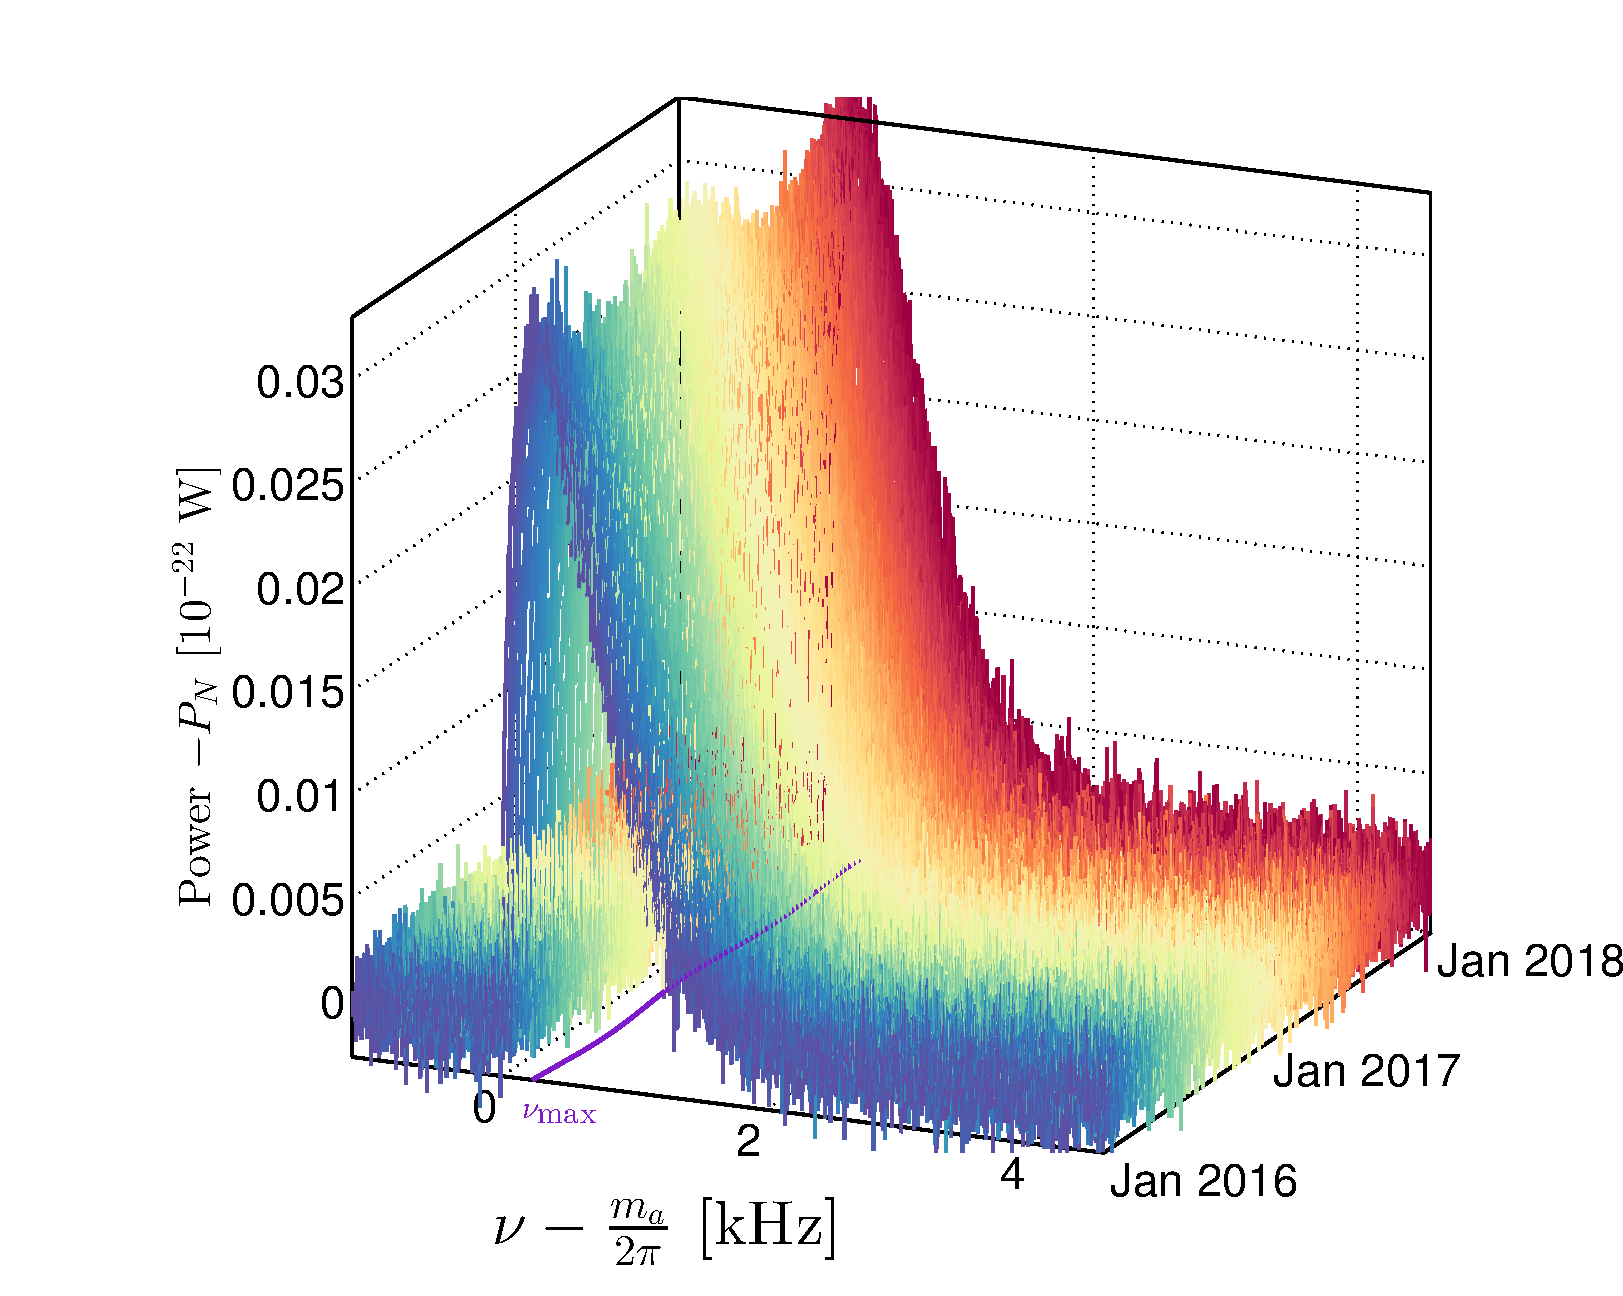
\includegraphics[width=0.8\textwidth]{Figures/axionpowerspectrum-eps-converted-to.pdf}\\
	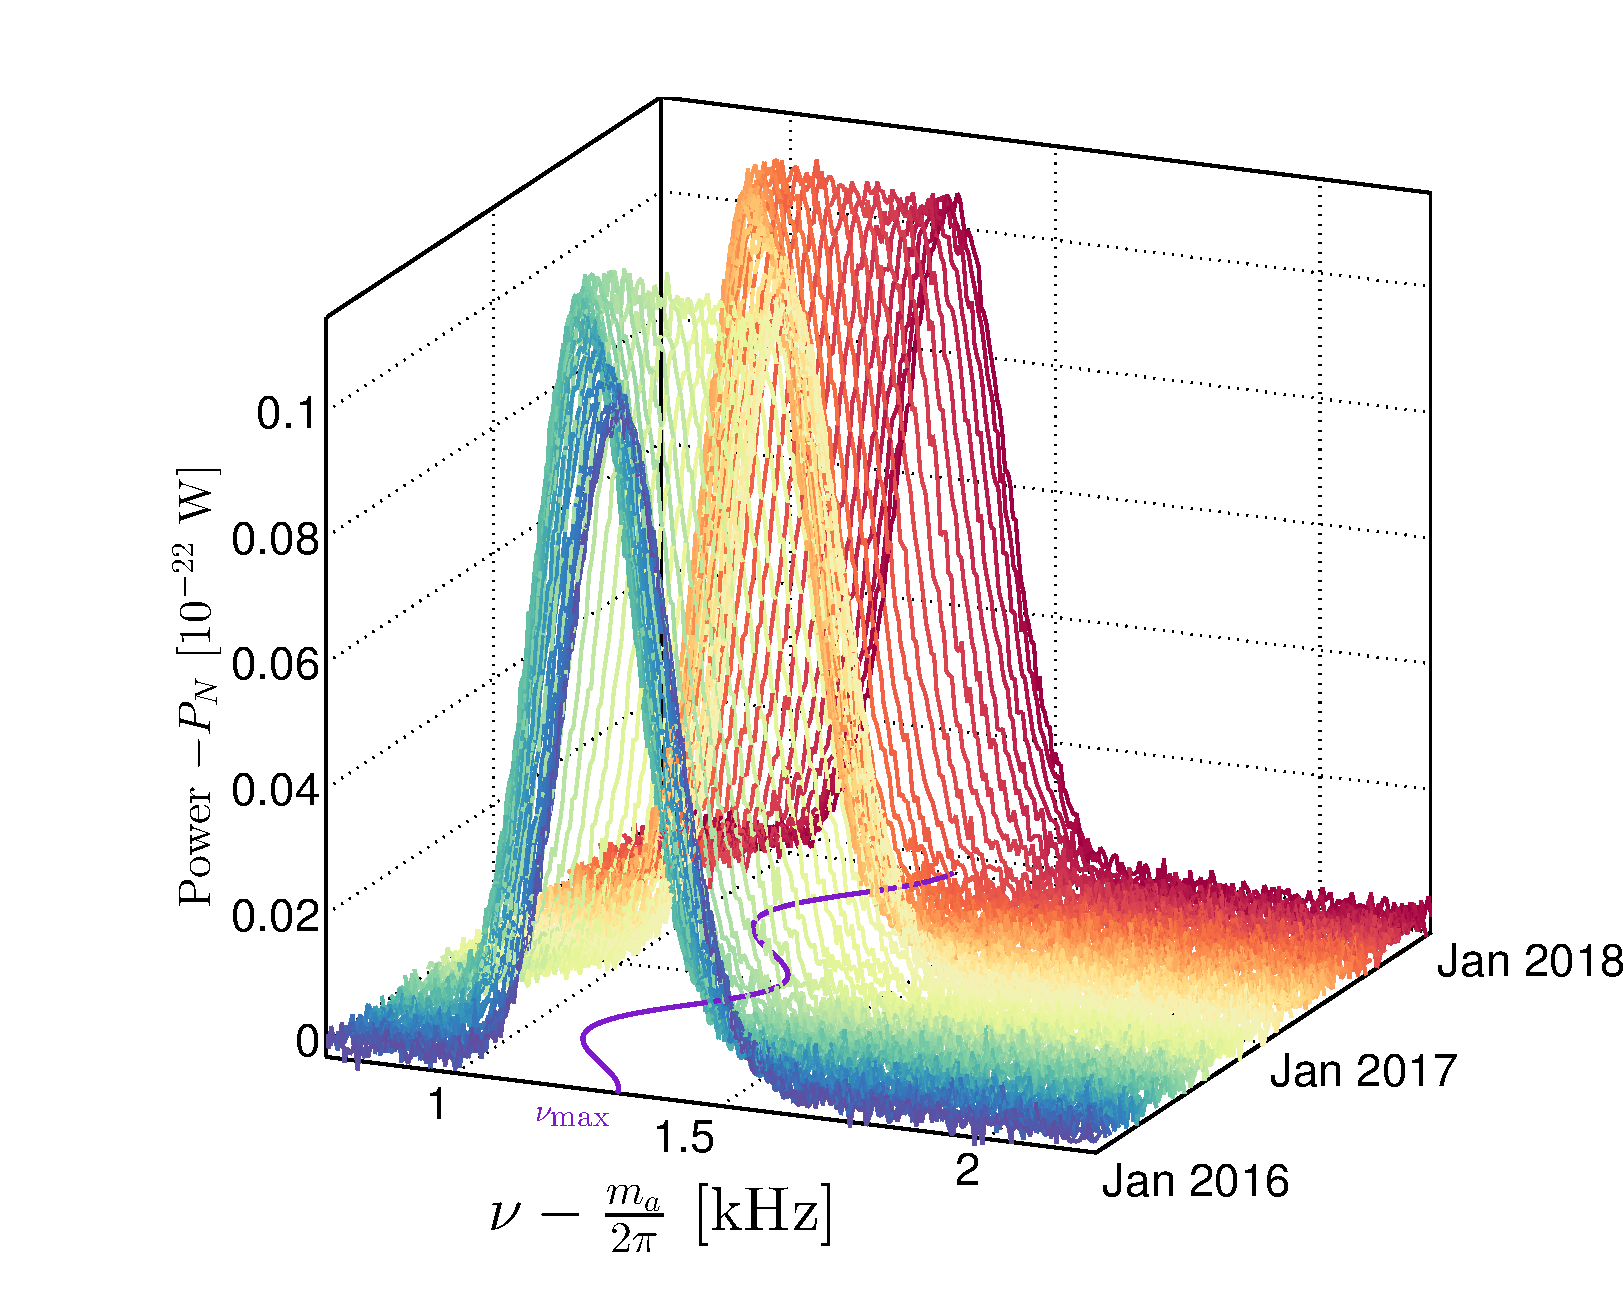
\includegraphics[width=0.8\textwidth]{Figures/axionpowerspectrum_stream-eps-converted-to.pdf}
    \caption[Example simulated axion power spectra as a function of time]{Example simulated power spectra as a function of time. Each line is the average power spectrum observed over a 10 day period. The top panel shows the spectra for a smooth Maxwellian halo and bottom for a pure tidal stream with parameter values displayed in Table~\ref{tab:partable}. The purple line in the frequency-time plane shows the evolution of the frequency at which the power is maximised: $2\pi\nu_\textrm{max} = m_a(1+ v_\textrm{lab}^2/2)$ and $2\pi\nu_\textrm{max} = m_a(1+ |\textbf{v}_\textrm{lab}+\textbf{v}_\textrm{str}|^2/2)$ for the Maxwellian halo and stream respectively.}\label{fig:axionpowerspectrum}
\end{center}
\end{figure}


Our simulation is an approximation of the current ADMX setup. We list a set of benchmark experimental parameters in Table~\ref{tab:partable}. The magnetic field strength, quality factor and noise temperature are roughly in line with what is currently achievable. For calculating the time dependence we also include the latitude and longitude of the experiment.

\begin{table}[t]\centering
\begin{tabularx}{0.8\textwidth}{c|ll}
    \hline \hline
\multirow{2}{*}{\bf Axion}
		& $m_a$ & 3.4671 $\mu$eV \\ 
		& $g_{a\gamma\gamma}$ & 10$^{-15}$ GeV$^{-1}$ \\ \hline 
\multirow{9}{*}{\bf Experiment}
		& $B_0$ & 8 T \\
		& $Q$ & 70,000 \\
		& $V$ & 220 l \\
		& $\Delta \tau$ & 0.2 s \\
		& $\tau$  & 10 days \\
		& $\tau_\textrm{tot}$ & 2 years \\
		& $T_S$ & 4 K \\
		& Latitude & $47.6553^\circ$ \\
		& Longitude & $-122.3035^\circ$ \\
		\hline \hline
    \end{tabularx}
  \caption{Benchmark axion and haloscope simulation parameters.}
\label{tab:partable}
\end{table}

In this section we will consider a hypothetical scenario in which the axion has been discovered after a successful low resolution scan over a wider mass range. Once the resonance has been found then an experiment can be performed at a single frequency. The running time of the experiment needs to be long enough to ensure that the signal-to-noise ratio is high but for our purposes also needs to be comprised of long timestream samples to obtain high frequency resolution in the resulting spectrum. 

For now we pick a benchmark set of particle parameters that lie in the QCD axion band: $\nu_a = 842.0$ MHz (= 3.4671 $\mu$eV) and $g_{a\gamma\gamma} = 10^{-15}$~GeV$^{-1}$. This choice evades existing constraints but is easily within the reach of ADMX given a long enough running time at the correct frequency. We use only a single particle benchmark in this study as we are placing the focus on the underlying astrophysical parameters. This is justified however because many of the conclusions are either independent of the choice in mass and coupling (provided the running time and resonant frequency are suitably adjusted) or have dependencies that are simple to explain from the scaling of the axion power. We discuss how one might extend our conclusions to other axion mass and coupling ranges in the Summary Sec.~\ref{sec:axions_summary}.

The sensitivity of a haloscope experiment is limited by the strength of the axion conversion power compared to the noise level. There are two main sources of background noise in resonant cavity experiments: the signal amplifier and the cavity walls. The cavity walls produce thermal blackbody photons (also known as Johnson noise) whereas the amplifiers produce electrical noise which depends on the precise technology, however both can be modelled as white noise~\cite{Daw:1998jm,Hotz:2013xaa,Brubaker:2016ktl}. The signal-to-noise ratio for a haloscope experiment of duration $\tau$, is set by the Dicke radiometer equation~\cite{Dicke:1946aa}
\begin{equation}
 SNR = \frac{P_a}{k_B T_S} \sqrt{\frac{\tau}{\Delta \nu_a}} \, ,
\end{equation}
where $\Delta \nu_a$ is the bandwidth of the axion signal and $T_S$ is the noise temperature.

Our mock experiment consists of a long total running time $\tau_{\rm tot}$ which is divided into separate time integrated bins of length $\tau$. Inside a given time bin we calculate a power spectrum which would correspond to the average of $\mathcal{N}$ Fourier transformed timestream samples of duration $\Delta \tau$. The Fourier transform of a given sample is a power spectrum with frequency resolution $\Delta \nu = 1/\Delta \tau$. The noise we simulate as Johnson white noise with temperature $T_S$ which has rms power $P_N = k_B T_S \Delta \nu$ inside a given frequency bin with an exponential distribution~\cite{Duffy:2006aa}. The noise power spectrum of the average of $\mathcal{N} = \tau/\Delta \tau$ individual exponential power spectra corresponding to the $\mathcal{N}$ Fourier transformed timestream samples then approaches Gaussian white noise in accordance with the central limit theorem. Hence our simulated noise inside the larger time bin $\tau$ is Gaussian white noise with mean value $P_N$ and standard deviation $P_N/\mathcal{N} = P_N/\sqrt{\tau \Delta \nu}$. The full dataset then consists of a total number of $N_\tau = \tau_{\rm tot}/\tau$ time integrated power spectra each of which consists of the axion power spectrum averaged over the time $\tau$ added to the Gaussian white noise. The major motivation for a long running time, aside from simply reducing noise, is to utilise the annual modulation due to $\textbf{v}_\textrm{rev}(t)$ which provides a Galactic perspective to the signal. 

We test our simulation by first generating a mock dataset and then attempting to reconstruct the input particle and astrophysical parameters with a maximum likelihood analysis. Two examples of such data are displayed in Fig.~\ref{fig:axionpowerspectrum} corresponding to two halo models, a smooth isotropic Maxwellian distribution and a pure stream (with parameter values listed in Table~\ref{tab:astrobenchmarks}). The annual modulation of the peak frequency is indicated by the purple line labelled $\nu_{\rm max}$.

We base our likelihood on a $\chi^2$ statistic which measures the offset between the observed value of power $P^{ij}_\textrm{obs}$, and the expected power (signal + rms noise) $P^{ij}_a + P_N$ in each bin, where $i$ and $j$ label frequency and time bins respectively,
\begin{equation}
 \chi^2 = \sum_{i = 1}^{N_\nu}\sum_{j = 1}^{N_t} \frac{\left(P^{ij}_\textrm{obs} - P^{ij}_a - P_N\right)^2}{\sigma^2_{N}} \, ,
\end{equation}
where the sums run over $N_\nu = (\nu_\textrm{max}-\nu_\textrm{min})/\Delta \nu$ frequency bins and $N_\tau = \tau_{\rm tot}/\tau$ time bins. The error $\sigma_N$ is given by the suppressed rms noise power $P_N/\sqrt{\tau \Delta \nu}$. We then construct a likelihood based on this statistic. Mathematically the likelihood as a function of a set of parameters given data $\mathcal{D}$ is,
\begin{eqnarray}
 \mathcal{L}(m_a,g_{a\gamma\gamma},P_N,\Theta | \mathcal{D}) = e^{-\chi^2/2}\, \mathcal{L}_N(P_N) \,,
\end{eqnarray}
where we assume $m_a$, $g_{a\gamma\gamma}$ and $P_N$ are free parameters. We also use the generic $\Theta$ to label a set of astrophysical parameters as we will perform tests with varying numbers of free parameters. The second term, $\mathcal{L}_N(P_N)$, parameterises the likelihood of the noise power which can be measured externally (although we set this to unity unless otherwise stated).


\section{Axion astronomy}\label{sec:axions_astronomy}
\subsection{Reconstructing basic parameters}\label{sec:axions_reconstruction}
In this section we use the simulation and analysis methodology described in Sec.~\ref{sec:axions_analysis} to attempt to reconstruct sets of input particle and astrophysics parameters. The aim is to quantify how accurately and with what correlations and degeneracies a future ADMX-like haloscope experiment would measure the local axionic dark matter distribution. In the following results we show 1- and 2-dimensional 68\% and 95\% confidence intervals/contours calculated using the profile likelihood, along with best fit parameters values which maximise the likelihood. The procedure we adopt mirrors that used in Chapters~\ref{chapter:directional}~and~\ref{chapter:nufloor}. We again explore the likelihood with nested sampling algorithms provided by {\sc MultiNest}, setting a tolerance of $10^{-3}$ and using $2\times 10^3$~-~$10^4$ live points depending on the number of parameters being reconstructed.

\begin{figure}
\begin{center}
	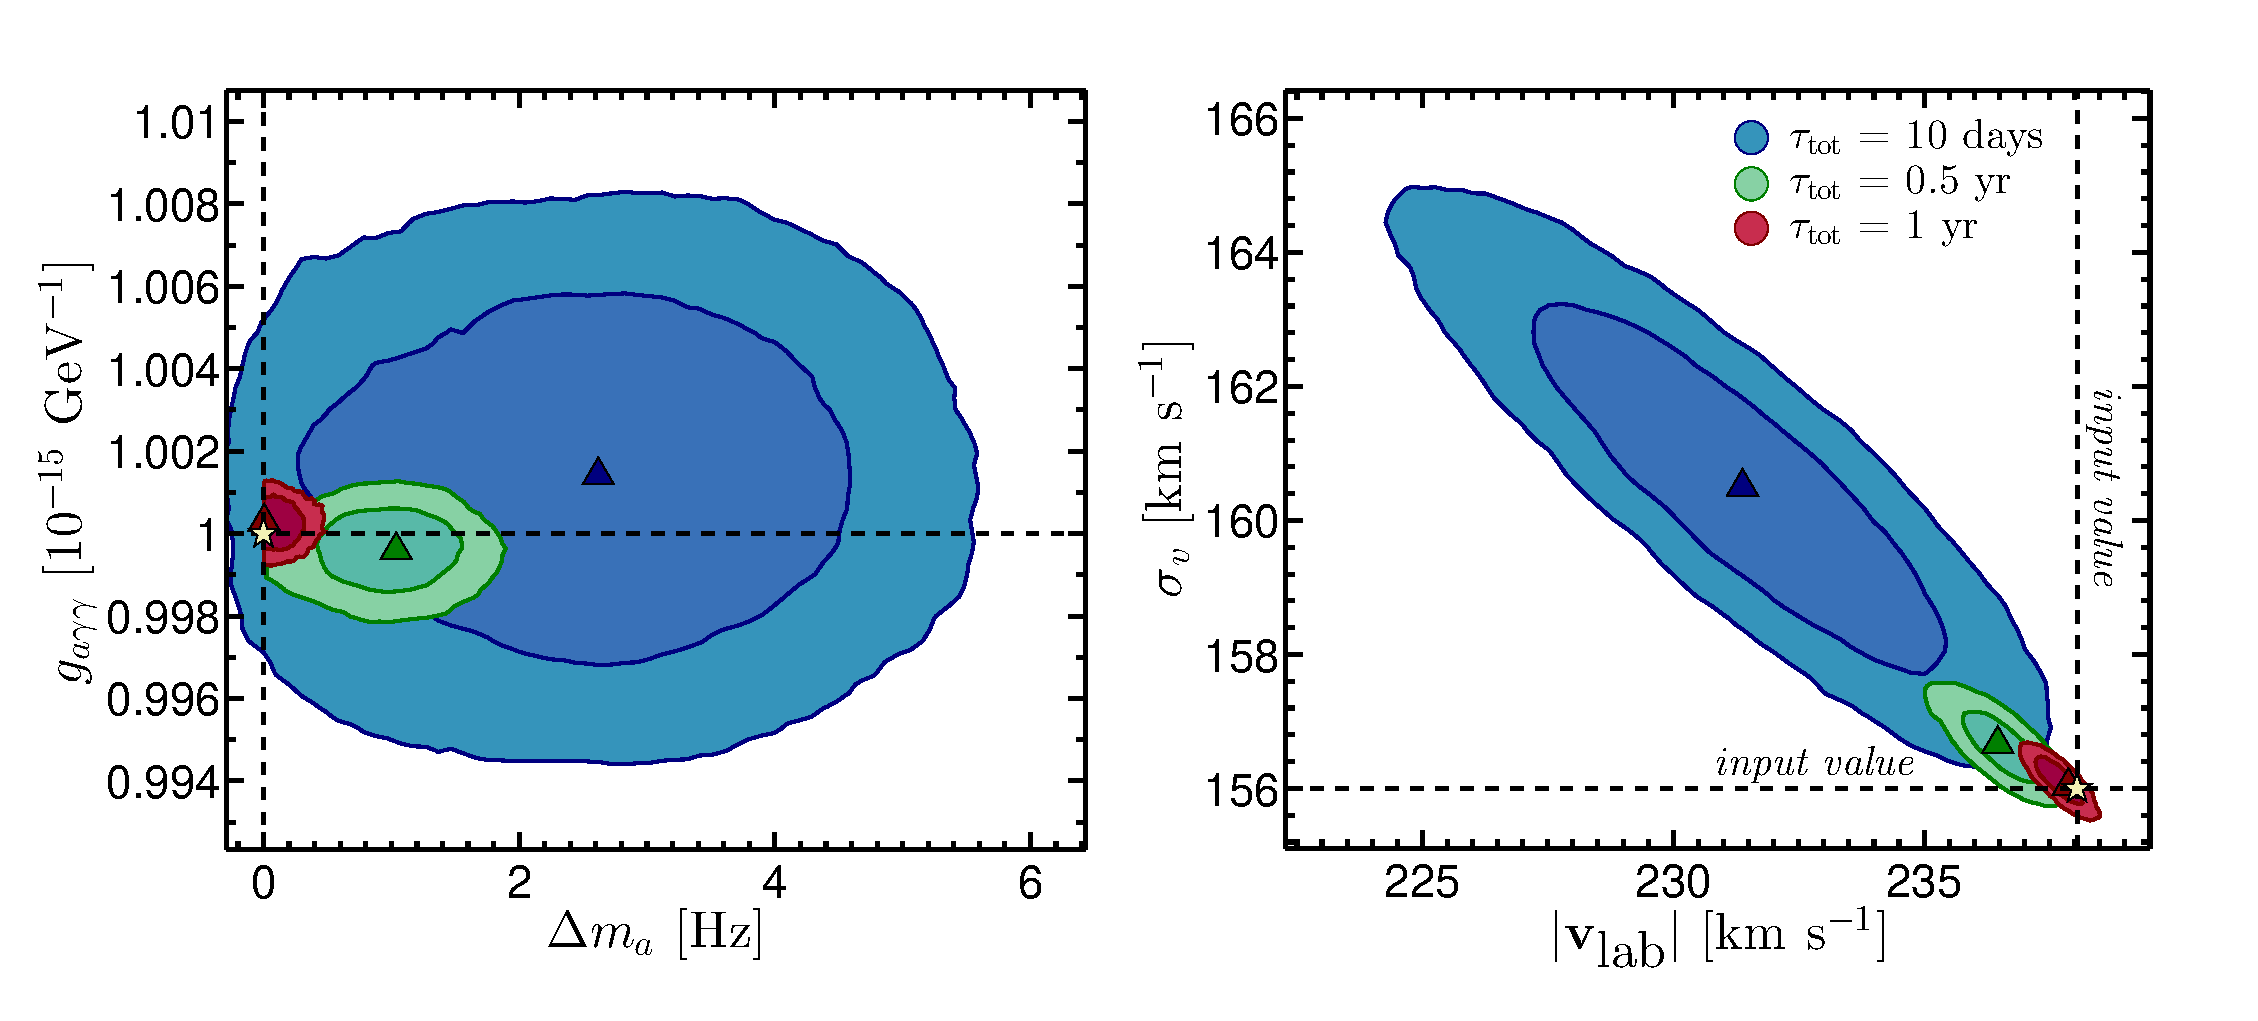
\includegraphics[width=0.99\textwidth]{Figures/axion_bench_recon.eps}
    \caption[Reconstructed axion mass, coupling and astrophysical parameters]{Reconstructed axion mass and coupling as well astrophysical parameters, $v_{\rm lab}$ and $\sigma_v$, for a smooth Maxwellian halo model. We show sets of 68\% and 95\% confidence level contours in the $m_a - g_{a\gamma\gamma}$ and $|\textbf{v}_{\rm lab}|-\sigma_v$ planes (left and right panels respectively). We express the axion mass as $\Delta m_a$ which has the true (input) value subtracted. The blue, green and red sets of contours correspond to the estimates with experiments of different durations: 10 days, half a year and 1 year respectively. The maximum likelihood values are indicated by triangles and the input values for the parameters are indicated by dashed lines and a yellow star.}\label{fig:axion_bench_recon}
\end{center}
\end{figure}
In Fig.~\ref{fig:axion_bench_recon} we show the reconstructed axion parameters $m_a$ and $g_{a\gamma\gamma}$ (left) and the astrophysical parameters $v_{\rm lab}$ and $\sigma_v$ (right). We show three sets of contours which correspond to experiments of different durations: 10 days, half a year and 1 year. The 10 day long experiment corresponds to a single time integrated bin of the 0.5 and 1 year long experiments. The annual modulation signal does not play a large role in constraining these parameters, hence the effect of increasing the experiment duration is to shrink the confidence intervals by a factor $\sqrt{\textrm{1 year}/\textrm{10 days}}$.  The axion mass and coupling can be measured to a high level of precision even with only 10 days of data taking, however there is some bias in the best fit values since the dataset consists of a single realisation of stochastic noise. The shapes of the contours are roughly one sided for masses $m>m_a$ due to the fact that the axion power spectrum is only non-zero for $\omega>m_a$. The astrophysical parameters can be measured to a high level of accuracy too. With a 1 year duration the level of precision would reach around the 1~km~s$^{-1}$ level, improving upon the accuracy of current astronomical observations~\cite{McMillan:2009yr}.

\begin{figure}
\begin{center}
	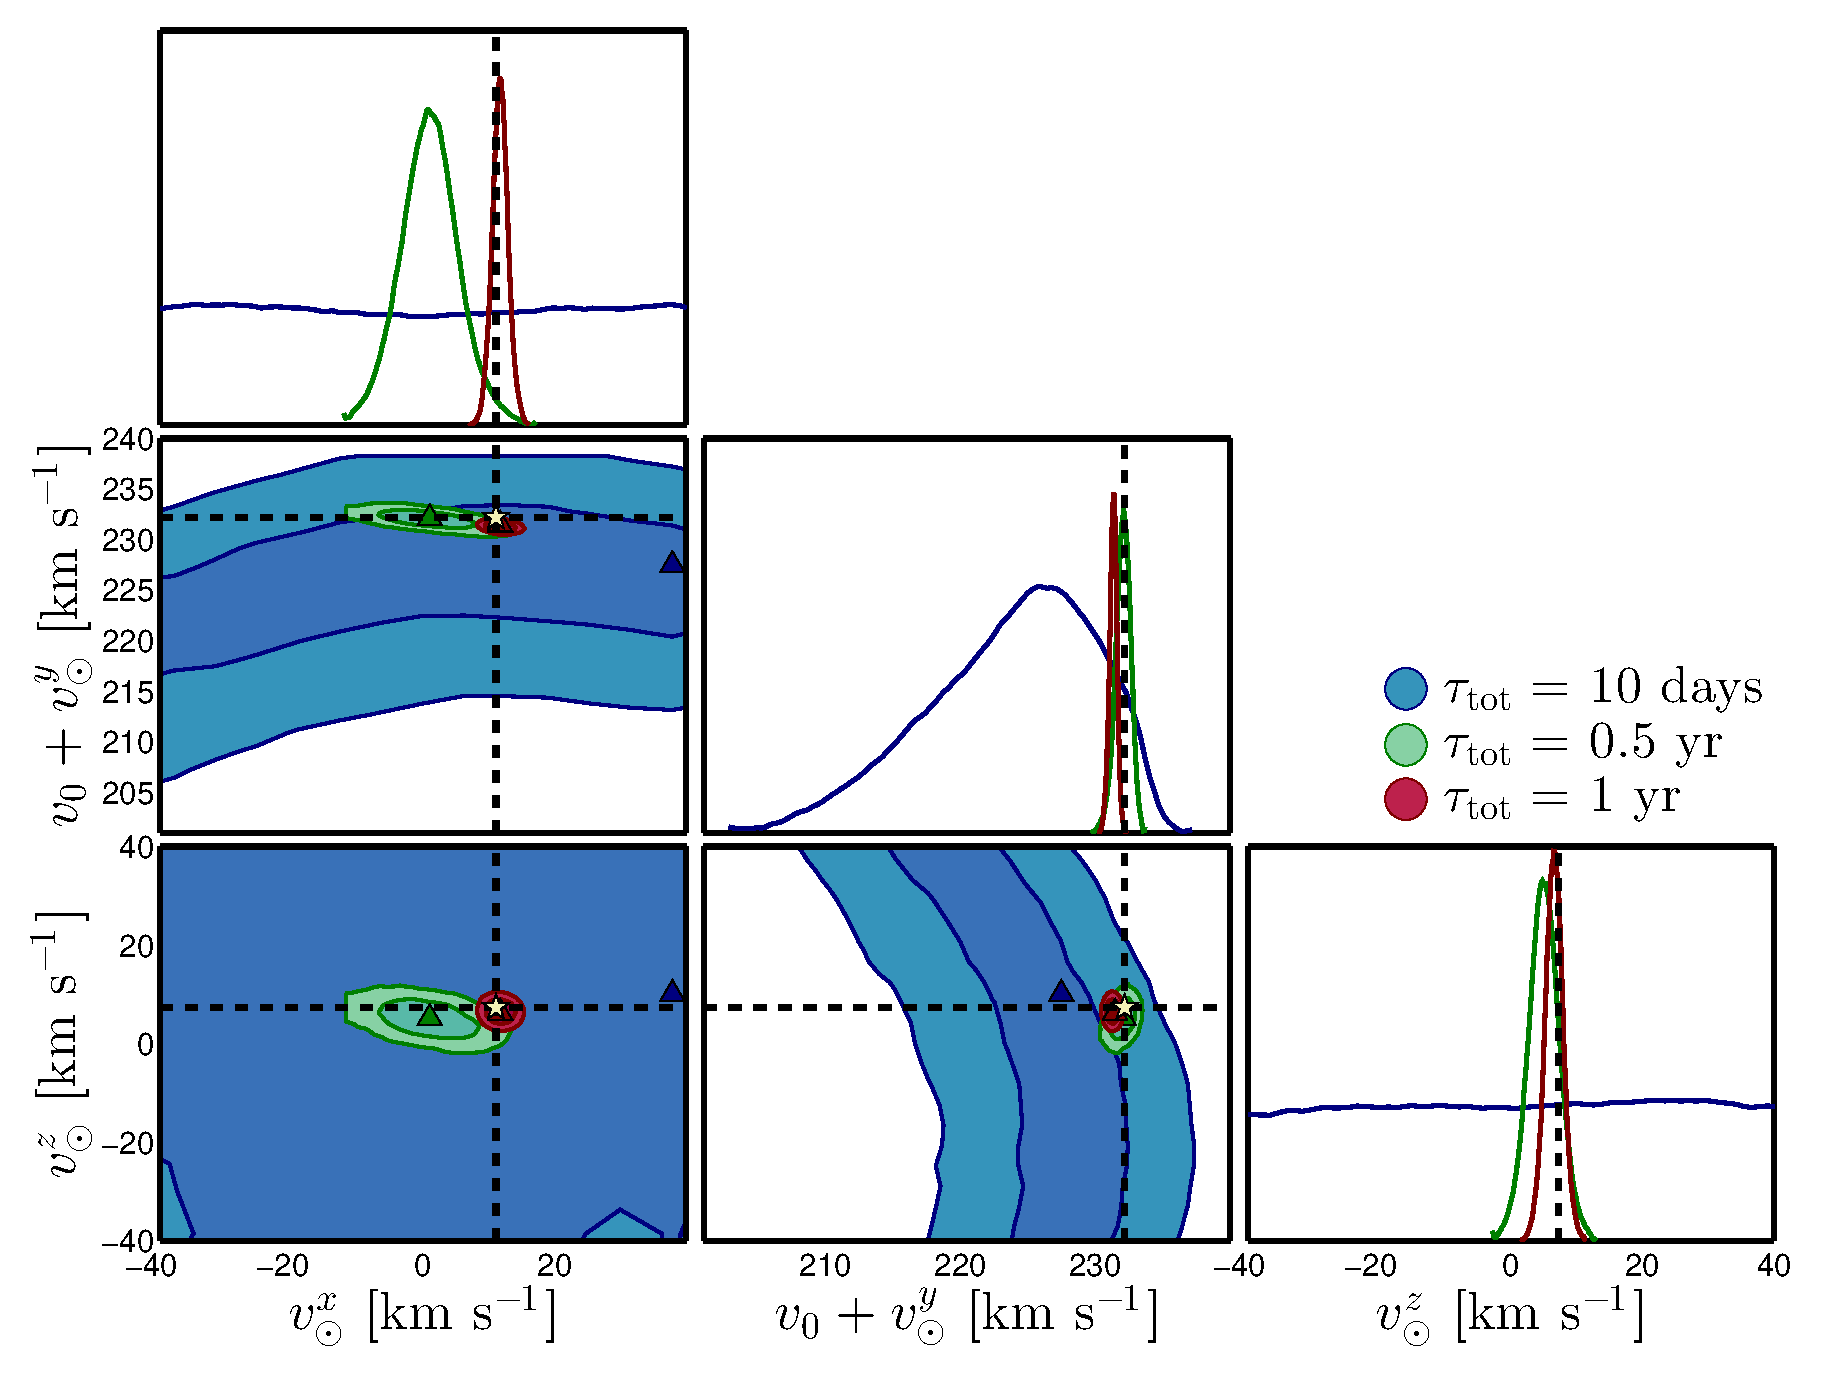
\includegraphics[width=0.9\textwidth]{Figures/vpec_reconstruction.eps}
    \caption[Reconstructed lab velocity components]{Reconstructed lab velocity components~$(v_\odot^x,~v_{0}~+v_\odot^y~,~v_\odot^z)$  at 68\% and 95\% confidence for three datasets of length 10 days, half a year and 1 year, indicated by blue, green and red sets of contours respectively. The maximum likelihood values are indicated by triangles and the true (input) values are indicated by dashed lines with a yellow star.}\label{fig:vpec_reconstruction}
\end{center}
\end{figure}
With a full annual modulation signal we can also access the 3-dimensional components of $\textbf{v}_\textrm{lab}$. However since $\textbf{v}_0$ and $\textbf{v}_\odot$ are summed in the Galactic frame we can only measure directly the $x$ and $z$ components of $\textbf{v}_\odot$. The $y$ component (i.e., that which lies along the direction of the rotation of the Milky Way) can only be measured in combination with the LSR speed $v_0$. In Fig.~\ref{fig:vpec_reconstruction} we show the measurement of these parameters for the same three experiment durations of 10 days, 0.5 and 1 year. Since the 10 day duration experiment consists only of a single time integrated bin we have no annual modulation signal and only the reconstruction of the largest component ($v_0+v^y_\odot$) is possible as this has the greatest influence on the shape of the spectrum. The remaining two components have essentially flat likelihoods as the single time bin spectrum is not sensitive to their values. However for longer durations with modulation in time, the measurement of all three components becomes possible. Even with only half a year of the annual modulation signal we can still make a measurement of the three components of $\textbf{v}_\textrm{lab}$ however as the signal-to-noise is lower the measurement is biased by particular large fluctuations, which in this example leads to the input values lying outside of the 95\% contour. With a full year of data however a very accurate measurement can be made with 95\% confidence intervals smaller than 5~km~s$^{-1}$ and the true values (indicated by dashed lines and stars) lying within the 95\% interval in all cases.

\begin{figure}
\begin{center}
	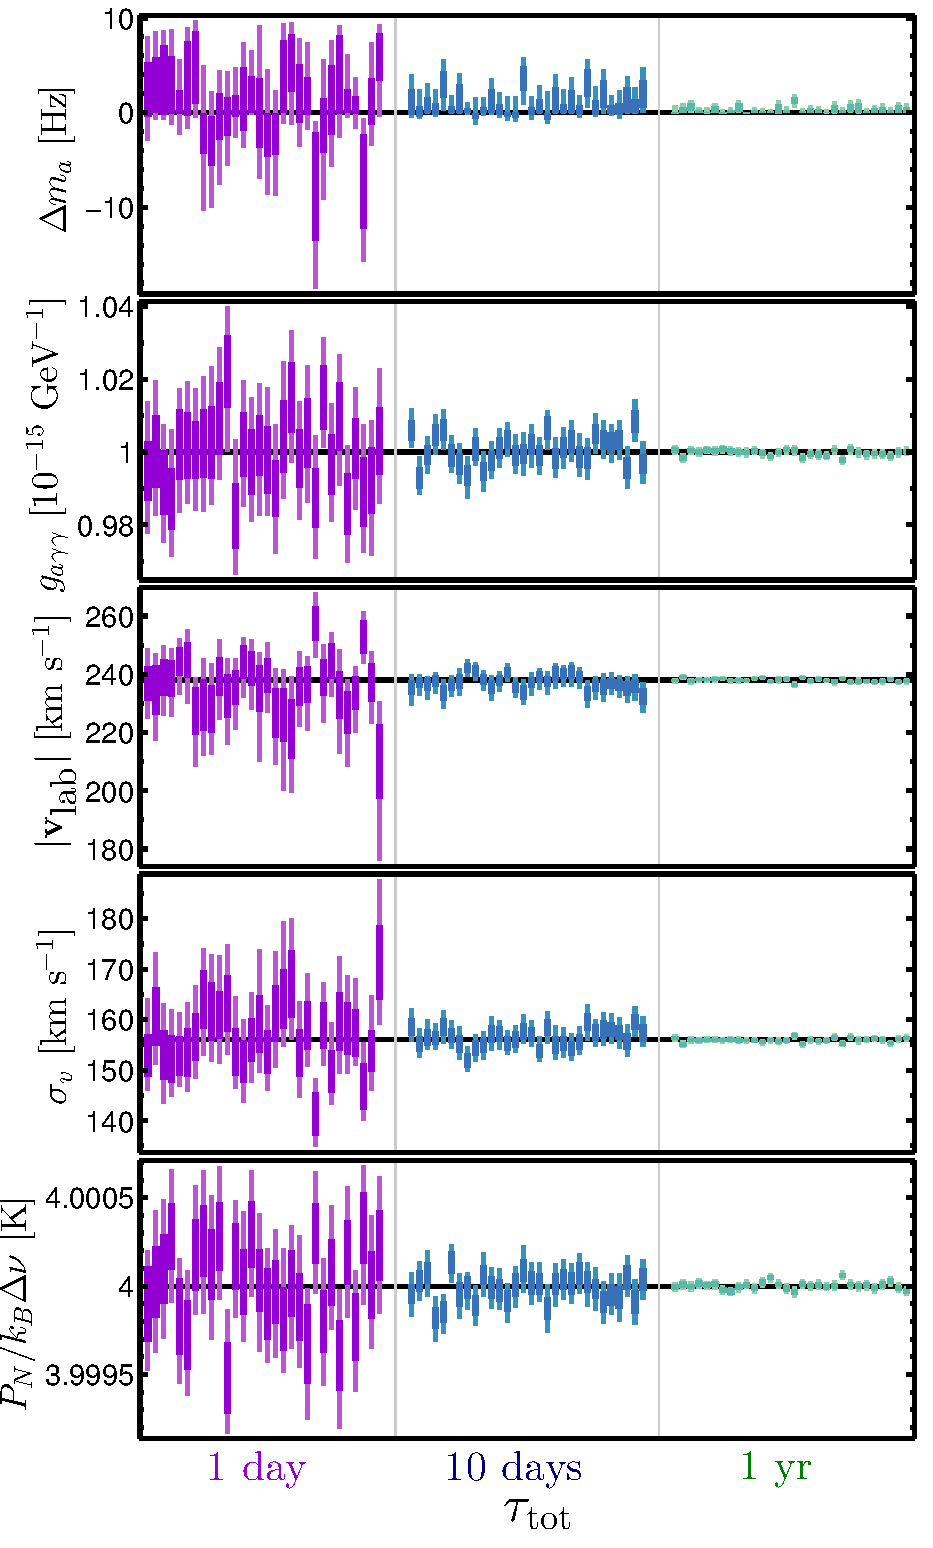
\includegraphics[width=0.8\textwidth]{Figures/reconstructionvstau-eps-converted-to.pdf}
    \caption[Multiple reconstructed axion parameters]{Reconstructed parameters for multiple stochastic data realisations. The 1 and 2 sigma error bars are shown for five parameters, from top to bottom, $m_a$, $g_{a\gamma\gamma}$, $|\textbf{v}_\textrm{lab}|$, $\sigma_v$ and the noise (which we express as $P_N/k_B \Delta \nu$). There are 30 sets of repeated measurements for 3 different experimental durations $\tau_{\rm tot} = $ 1 day, 10 days and 1 year (from left to right).}\label{fig:reconstructionvstau}
\end{center}
\end{figure}
Finally in Fig.~\ref{fig:reconstructionvstau} we show the 1 and 2 sigma error bars for various parameter measurements as a function of the total experiment duration $\tau_{\rm tot}$. We use three experiment durations from 1 day to 1 year and for each we repeat the experiment 30 times with different randomly generated noise in each to demonstrate the sensitivity to the individual data realisation. As shown in Figs.~\ref{fig:axion_bench_recon} and \ref{fig:vpec_reconstruction} the short duration experiments as well as setting much weaker measurements are also biased by the particular data causing some reconstructions to lie further than 2 sigma away from their input values. In the case of the axion mass we expect one-sided measurements due to the one-sided nature of the power spectrum. This is the case for 10 day and 1 year durations, however for the 1 day duration we see multiple experiments reconstruct a mass smaller than the input mass due to large noise fluctuations in bins slightly below the axion mass. Interestingly for the longer duration experiments the constraint on the axion mass reaches a level smaller than a single frequency bin (5 Hz), this is because the shape of the power spectrum and the annual modulation signal also provide additional information about $m_a$. The size of the error bars for the remaining parameters decrease roughly as $1/\sqrt{\tau_{\rm tot}}$ and for durations long enough to exploit the annual modulation signal we see a significant decrease in the scatter in the reconstructed values over different realisations of the experiment. This means that a future experiment of this kind would be able to make fine measurements of the axion particle parameters in conjunction with astrophysical parameters and with no major biases.


\subsection{N-body data}\label{sec:axions_nbody}
We can source more realistic examples of dark matter distributions from N-body simulations of Milky Way-like halos. These might more accurately reflect the inhomogeneities and anisotropies that will likely be present in a real dark matter halo. This is of particular interest for a high resolution axion experiment because, as shown in the previous subsection, it is far more sensitive to astrophysical parameters than standard axion searches and WIMP direct detection. 

We use data from the Via Lactea II (VL2)~\cite{Diemand:2007qr} simulation and select 200 analogue Earth locations at a Galactic radius of 8~kpc and calculate a velocity distribution from all particles contained within 1 kpc spheres centred on each of these locations (we also enforce that no spheres overlap). Although there are more recent hydrodynamic simulations that will better reflect a Milky Way-like dark matter distribution, the VL2 data is sufficient for the illustrative examples we show here and will not change the general conclusions.

\begin{figure}
\begin{center}
	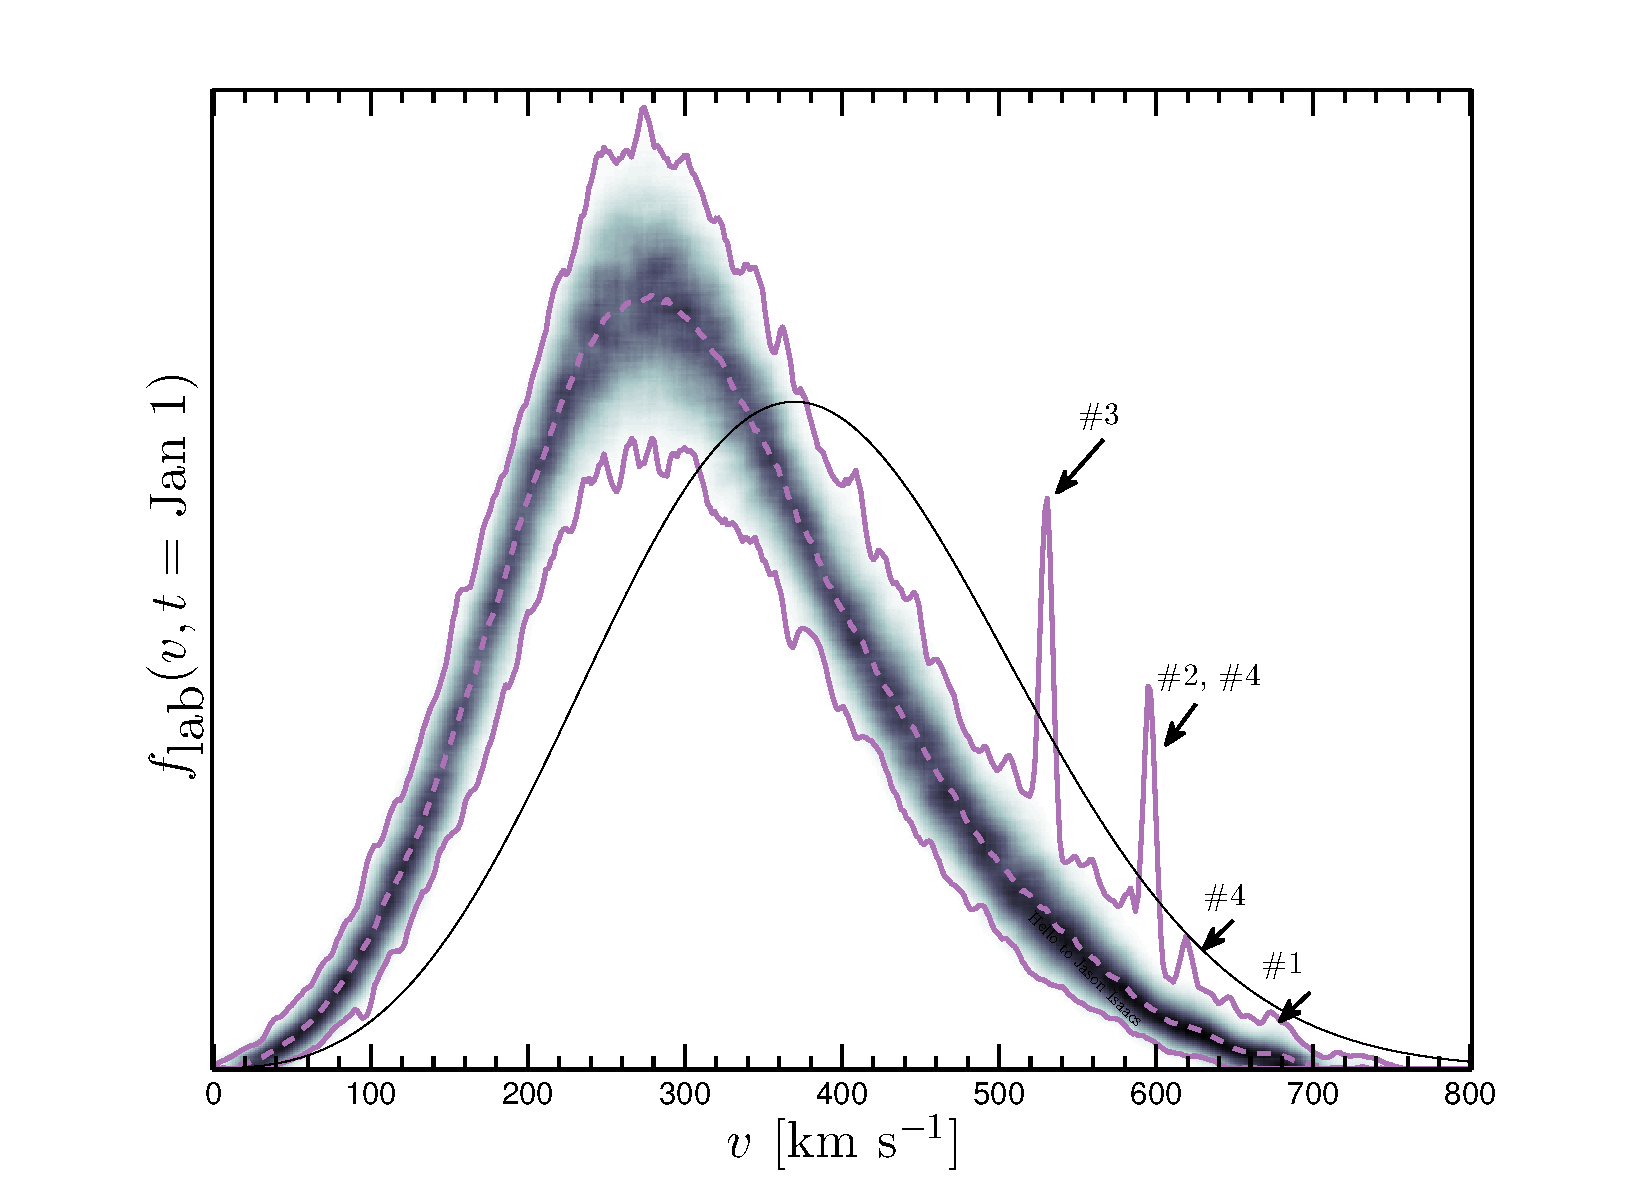
\includegraphics[width=0.8\textwidth]{Figures/vl2speeddist-eps-converted-to.pdf}
    \caption[VL2 lab frame speed distributions]{Set of laboratory frame speed distributions of the 200 samples chosen from the VL2 simulation. The shaded regions indicate the range of $f(v)$ values for a given $v$. The solid purple lines indicate the maximum and minimum values of $f(v)$ and the dashed line is the mean distribution over all samples. The black line is the SHM Maxwellian with parameters from Table~\ref{tab:partable}. We label particular samples containing prominent streams.}\label{fig:vl2speeddist}
\end{center}
\end{figure}
We display the range of these 200 velocity distributions in Fig.~\ref{fig:vl2speeddist} with certain samples labelled which contain a significant substructure component. These are of particular interest here as kinematically localised streams travelling with velocities at an angle to the lab velocity would give rise to varied annual modulation signals. We label these samples from \#1 - \#4.

We calculate the axion conversion power spectrum in the same way as before but we substitute the analytic $f(\omega)$ with a discretised version calculated by binning particle velocities with a bin size roughly corresponding to the frequency resolution of the experiment. Importantly for each time bin at $t$ we rotate all particle velocities into the laboratory frame with the time dependent Galactic to laboratory transformation detailed in Appendix~\ref{app:labvelocity}. We must also boost all particle velocities by $\textbf{v} \rightarrow \textbf{v} - \textbf{v}_\textrm{lab}(t)$.

\begin{figure}
\begin{center}
	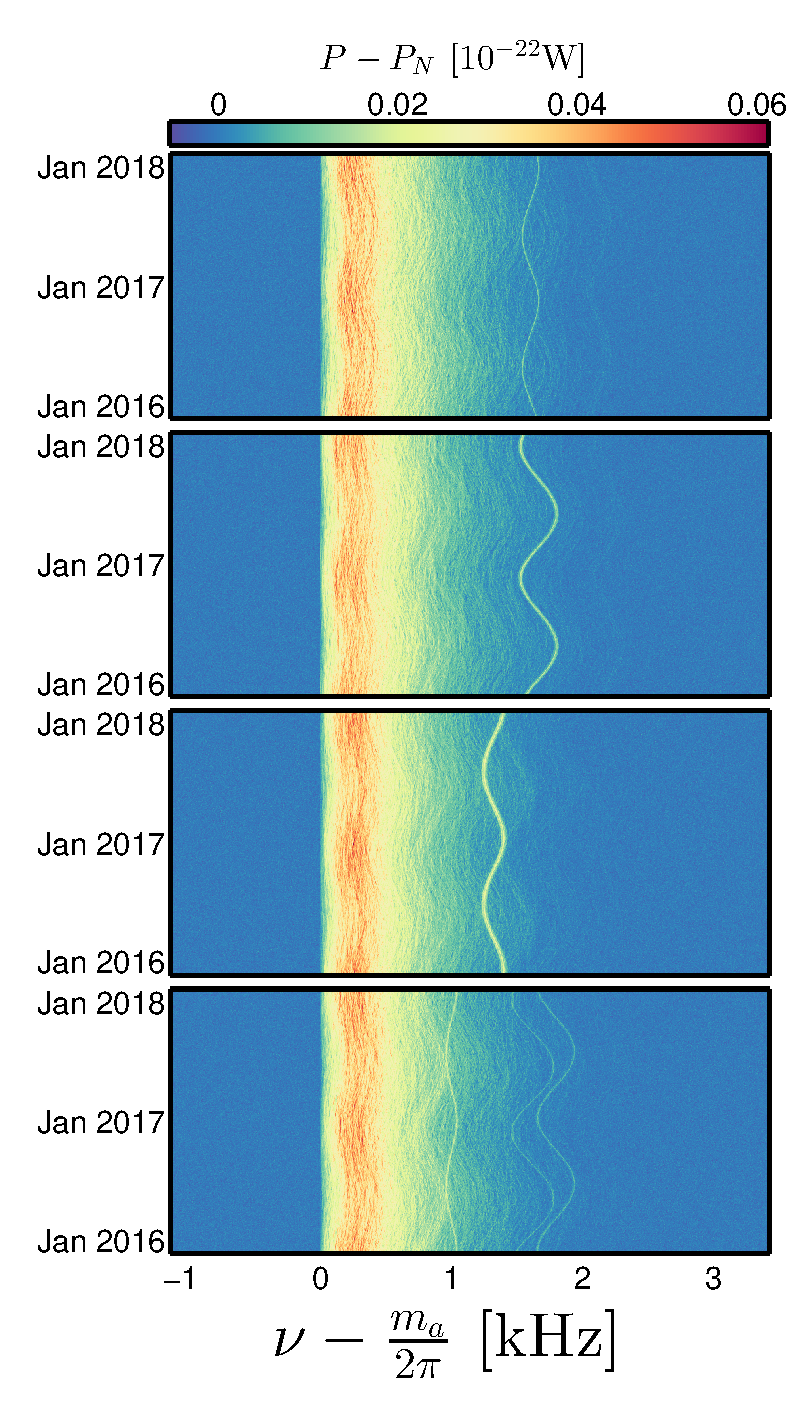
\includegraphics[width=0.49\textwidth]{Figures/vl2_powerspectra.eps}
	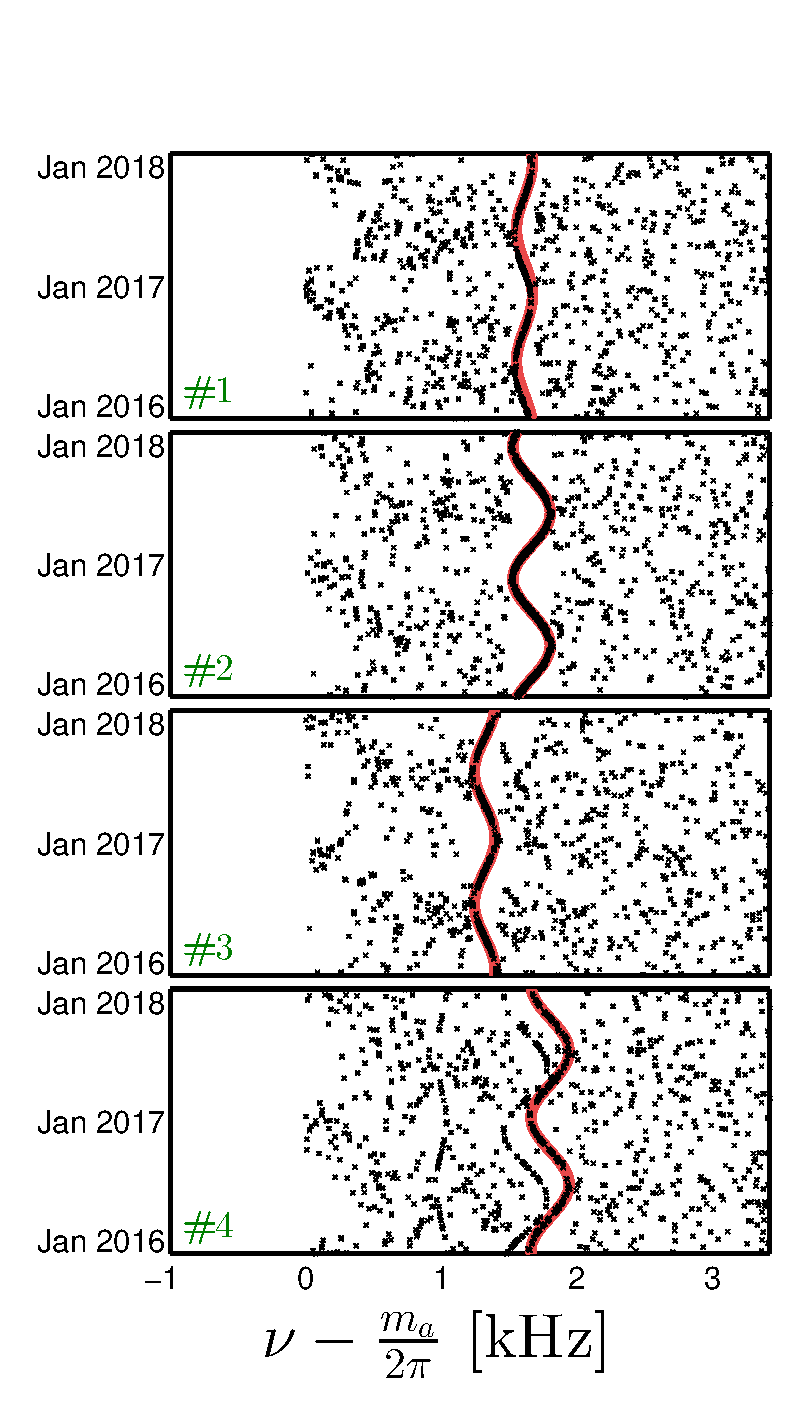
\includegraphics[width=0.49\textwidth]{Figures/vl2_reduced.eps}
    \caption[VL2 axion conversion power spectra]{{\bf Left:} Axion conversion power spectra for a selection of four Earth-radius dark matter velocity distributions from the VL2 simulation. In each of the four examples the power spectrum has the amplitude of the noise power ($P_N$) subtracted and is displayed as a function of time. The frequency axis is presented as the difference between the photon frequency and the axion mass. {\bf Right:} The same set of power spectra after performing the various cuts detailed in the text. The remaining points show fluctuations in the axion power spectra after the time independent components have been subtracted. The best fit to Eq.~(\ref{eq:sinefit}) is shown as a red line.}\label{fig:vl2_powerspectra}
\end{center}
\end{figure}
In Fig.~\ref{fig:vl2_powerspectra} we show a selection of four axion conversion power spectra for a range of sample VL2 velocity distributions (the same selection as labelled in Fig.~\ref{fig:vl2speeddist}). The four examples are selected because they contain significant substructure components in the form of streams. These show up in the power spectra as sinusoidally modulating features in time. Some examples, such as \#2 and \#3, having single dominating streams whereas others, such as \#4, possess multiple streams with different amplitudes and phases. 

We can parameterise the frequency dependence of the modulating streams with the function
\begin{equation}\label{eq:sinefit}
\nu(t) = \nu_1 \sin\left(2\pi\left(\frac{t-t_0}{\textrm{1 year}}\right)\right) + \nu_0 \,.
\end{equation}
In principle the three parameters of this function are related to the three Galactic frame components of the stream velocity, although this will not be a one-to-one mapping. The frequency of the stream modulation $\nu(t)$ is proportional to the quantity $|\textbf{v}_\textrm{str}-\textbf{v}_\textrm{lab}(t)|^2$. 

We can extract substructure components from the pseudodata we have presented here by searching for sinusoidally modulating features that have a period of 1 year (whilst also fitting for the function Eq.~(\ref{eq:sinefit})). First we can reduce the data by subtracting the time averaged spectrum and then dividing by the standard deviation of the remaining fluctuations. Next we perform a cut over bins with power fluctuations below a certain level of significance leaving a series of points which if the stream component is large enough will retain the sinusoid modulation. The resulting data points for each example are shown in the left hand panels of Fig.~\ref{fig:vl2_powerspectra}. These data points can then be fit to a model for the stream. We again use the same Maxwellian form for the stream velocity distribution with power spectrum shown in the lower panel of Fig.~\ref{fig:axionpowerspectrum}. Whilst the stream is unlikely to be perfectly described by a Maxwellian, any deviations will be smaller than the error induced by the finite frequency resolution and noise fluctuations. 

\begin{figure}
\begin{center}
	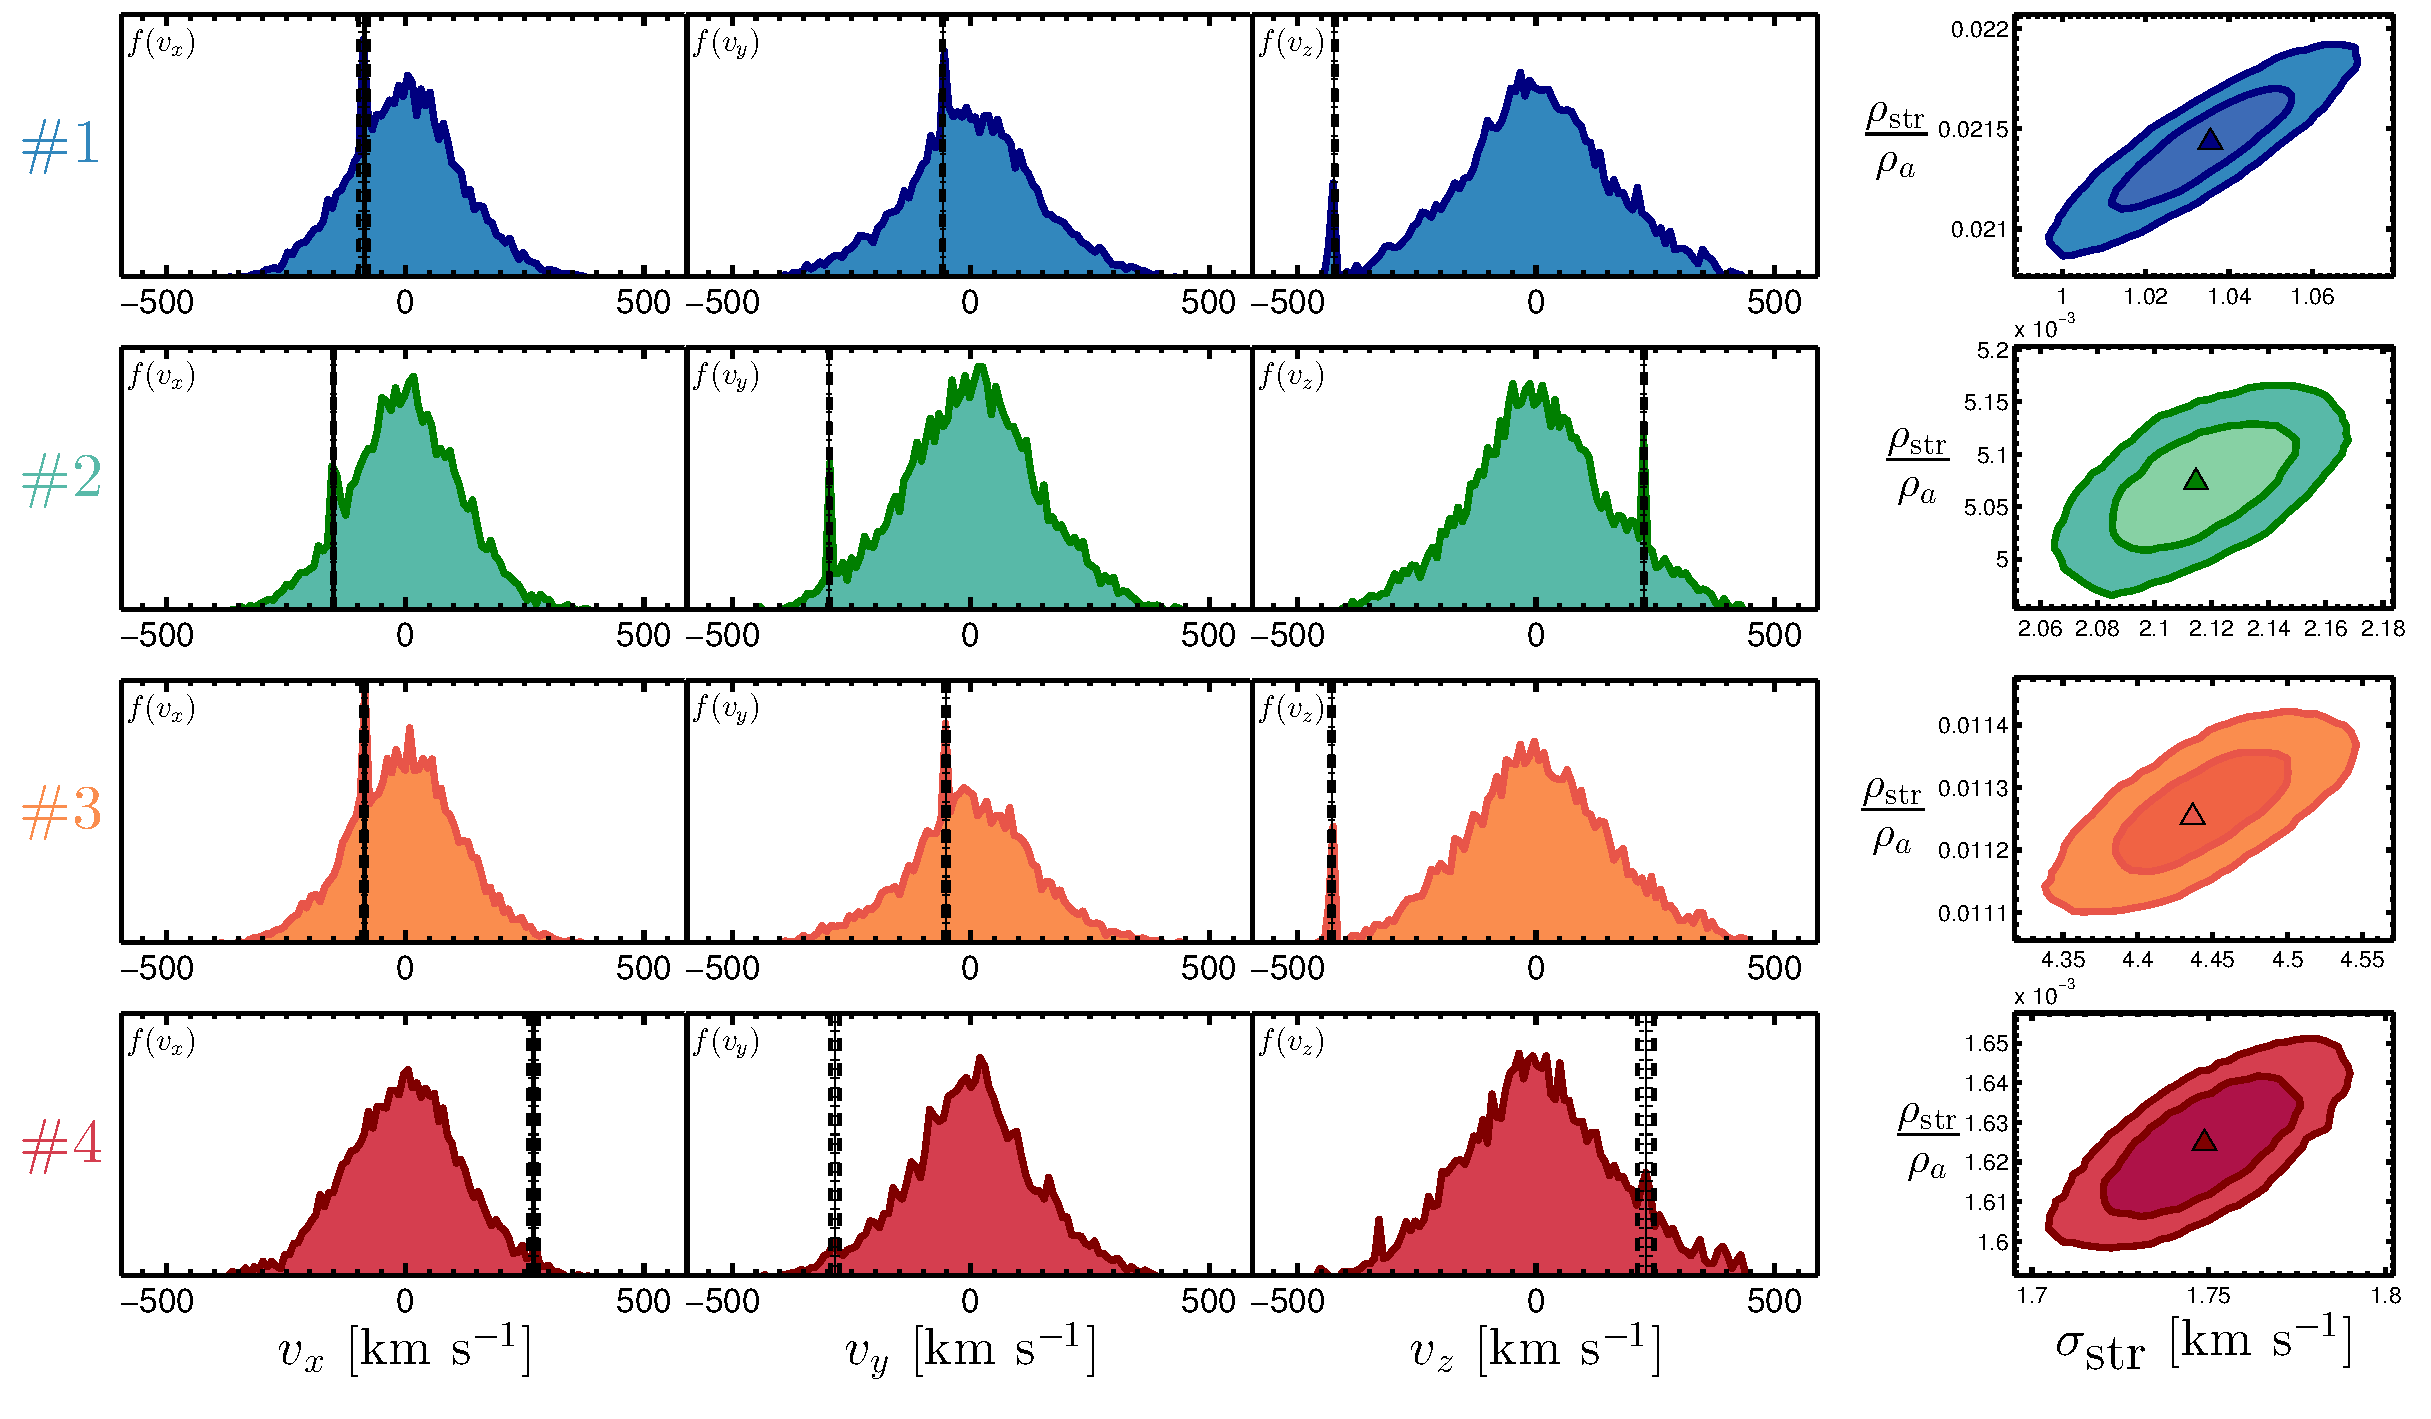
\includegraphics[width=0.95\textwidth]{Figures/stream_estimate-eps-converted-to.pdf}
    \caption[Measuring axion stream velocity]{Measurements of stream velocity (vertical black lines) and intervals at the 68\% and 95\% confidence level (dotted and dashed lines respectively) for each of the four sample VL2 velocity distributions. The 1-dimensional speed distributions in each Galactic coordinate $(v_x,v_y,v_z)$ correspond to the first three columns. Each row corresponds to the four sample distributions chosen. The final column shows each reconstruction in the stream density - dispersion plane.}\label{fig:stream_estimate}
\end{center}
\end{figure}
A given stream is described by its density $\rho_\textrm{str}$, dispersion $\sigma_{\rm str}$, and three components of velocity $\textbf{v}_\textrm{str}$ making a total of five parameters. Since we have a method for extracting the stream from the data, we can use the data that remains once the stream is removed to fit for the axion, halo and lab velocity parameters and break the degeneracy with the stream parameters. In Fig.~\ref{fig:stream_estimate} we show the reconstructed stream velocities for the four samples displayed in Fig.~\ref{fig:vl2_powerspectra}. Note that in all cases all components of the stream velocity can be reconstructed to high accuracy due to the prominence of the annual modulation signal. This is because the three components of the velocity can all be independently measured with the use of the phase, mean frequency and amplitude of the modulation in Eq.~(\ref{eq:sinefit}), although this relationship is nonlinear due to the transformation from the Galactic to the laboratory frame.

Also in Fig.~\ref{fig:stream_estimate} we show the measurement of stream density fraction and dispersion for each sample. Because the density fraction and dispersion are respectively related to the power amplitude and width of the modulating feature, a reconstruction of these parameters is possible in addition to the velocity components. The four samples we have considered here all have relatively large stream contributions which aids the measurement of these parameters. For weaker streams it is likely that longer duration experiments would be required to increase the signal-to-noise. Here the lowest density stream that is detectable with our method is set by the power with respect to the level of noise. Furthermore we have not explored the full stream velocity parameter space with these four examples. It is likely that the accuracy of the reconstruction will be dependent on the direction of the stream with respect to the direction of the lab velocity. Additionally with higher signal-to-noise examples it should also be possible to reconstruct more than one stream (as in sample \#4). We leave these issues however to future work.



\subsection{Axion miniclusters}\label{sec:axions_miniclusters}
There has been sustained interest in small high density bound structures of axions called miniclusters (see e.g. Refs.~\cite{Hogan:1988mp,Kolb:1993zz,Kolb:1993hw,Kolb:1994fi,Kolb:1995bu,Berezinsky:2013fxa,Tinyakov:2015cgg,Fairbairn:2017dmf}). Miniclusters are formed in the early Universe from density perturbations in the axion field. Perturbations forming miniclusters can result from various types of non-linear dynamics involved with axion oscillations such as vacuum misalignment or the decay of axion defects such as strings and domain walls~\cite{Chang:1998tb}. Previous work has predicted the existence of up to $\sim 10^{10}~\textrm{pc}^{-3}$~\cite{Tinyakov:2015cgg} locally if all of the dark matter was in the form of miniclusters, though a direct encounter would occur less than once every $10^5$ years~\cite{Kolb:1994fi}. Through close interactions with stars however axion miniclusters would become tidally disrupted leading to a network of streams wrapping the Milky Way (possibly in addition to a smooth component of the dark matter halo). The miniclusters will pass through the stellar disk many times over the age of the Milky Way ($t_{\rm MW} \sim 12$~Gyr). It has been estimated in Ref.~\cite{Tinyakov:2015cgg} that a small population of disrupted miniclusters would lead to several streams along the path of the Earth through the Galaxy that are large enough to induce an enhancement in the observed total power. The final result of Ref.~\cite{Tinyakov:2015cgg} is a value for the number of expected stream crossings with a density larger than the local smooth halo density $\rho_a$, which is interpreted as an amplification factor. However if the axion minicluster streams are an additional component to the smooth component then the stream density does not need to be larger than the local density to provide an enhancement to the signal. Since the velocity dispersion of the minicluster streams is extremely small compared to the halo ($\sim10^{-4}$~km~s$^{-1}$ $\ll 10^{2}$~km~s$^{-1}$), in a high resolution axion experiment all of the minicluster stream axions would convert to photons in a small number of frequency bins. Hence for a minicluster stream to be observable we simply need the total power from the stream to be larger than the power over a few bins.

Individual miniclusters are parameterised by the density contrast in the axion field, $\Phi = \delta \rho_a / \rho_a$ which is a number typically of order unity. The distribution of values of $\Phi$ found from the simulations of Ref.~\cite{Kolb:1995bu} appears to follow a function similar to $f_\Phi(\Phi) \sim \Phi^{0.75} e^{-\Phi}$ which we will use as an approximation. The mass of a minicluster is set by the total mass of axions inside the Hubble radius around the time when axion oscillations begin, $M_1 \sim 10^{-12}\, M_\odot$\footnote{This mass range is currently still allowed by lensing bounds~\cite{Zurek:2006sy}.}. Ref.~\cite{Kolb:1995bu} states that the distribution of minicluster masses is concentrated tightly around a large fraction of this mass.

Solving for the collapse of a spherical region with density contrast $\Phi$ and evolving through cosmic time to the present day gives a range of minicluster densities, 
\begin{equation}
\rho_{\rm mc}(\Phi) \simeq 7 \times 10^6 \, \Phi^3 (1+\Phi) \, \textrm{GeV cm}^{-3} \, .
\end{equation}
We assume that the miniclusters are spherically symmetric with central density $\rho_{\rm mc}(\Phi)$ and radius $R_{\rm mc}(\Phi,M)$. We assume a Maxwellian distribution for the speeds of axions inside a minicluster with a dispersion set by the virial velocity $\sigma_{\rm mc}(\Phi,M) = \sqrt{G M/R_{\rm mc}(\Phi,M)}$. Inspired by Ref.~\cite{Zurek:2006sy}, we assume the miniclusters have a power law density profile with $\rho \propto r^{-9/4}$ for $r<R_\textrm{mc}$. 

The number of streams expected at the Solar radius results from evolving the initial distribution of axion miniclusters through the age of the Galaxy to today. Each time the minicluster crosses the stellar disk there is a probability that it will encounter a star close enough to become disrupted. Following previous calculations of this type~\cite{Goerdt:2006hp,Schneider:2010jr}, Ref.~\cite{Tinyakov:2015cgg} gives the probability of a particular minicluster being disrupted,
\begin{equation}\label{eq:disruptprob}
P(\Phi) = 8\pi n S_{\perp} \frac{G R_{\rm mc}(\Phi,M)}{v \sigma_{\rm mc}(\Phi,M)} \,,
\end{equation}
where here $v$ is the orbital speed of the minicluster, and $n$ the number of crossings of the stellar disk the minicluster undergoes. This calculation has already averaged over an isotropic distribution of minicluster trajectories and has been written in terms of the stellar contribution to column density in the direction perpendicular to the disk, $S_{\perp} = 35 \,\textrm{M}_\odot\, \textrm{pc}^{-2}$~\cite{Kuijken:1989hu}. Given this, we can just use miniclusters with circular orbits intersecting the Solar position ($r_\odot$) to evaluate the number of crossings over the age of the Galaxy ($t_{\rm MW}$) to be roughly $n \sim 2 \, t_{\rm MW}/t_{\rm orb} \sim v \,t_{\rm MW} / \pi r_\odot \sim 100$. Note that the dependence on $v$ drops out of Eq.~(\ref{eq:disruptprob}). This is because although faster miniclusters cross the stellar disk more frequently ($\propto v$), they are also less likely to encounter a star during a given crossing ($\propto 1/v$). We also note that $P(\Phi)$ has no dependence on $M$ since $R_{\rm mc}(\Phi,M)$ and $\sigma_{\rm mc}(\Phi,M)$ are both proportional to $M^{-1/3}$.
 
A stream can be specified alone by four parameters: the density contrast $\Phi$ and mass $M$ of the original minicluster, the age of the stream $t$, and the orbital velocity of the minicluster/stream, $\textbf{v}$. All other parameters can be derived (we indicate dependence on each by parentheses). Once a minicluster is disrupted by a star it will begin to leave a trail of axions along its orbit, the length of which will stretch linearly with time as the cluster orbits the Galaxy $L \sim \sigma_{\rm mc} t$. Assuming the stream retains the original radius of the minicluster and is simply deformed from a sphere of radius $R_{\rm mc}$ into a cylinder of length $L$, the density of the axions for a minicluster stream of age $t$ is, 
\begin{equation}\label{eq:mcstreamdensity}
\rho_{\rm str}(\Phi,M,t) = \rho_{\rm mc}(\Phi) \frac{\frac{4}{3}R_{\rm mc}(\Phi,M)}{\sigma_{\rm mc}(\Phi,M) t} \, .
\end{equation}

Reference~\cite{Tinyakov:2015cgg} calculates the number of expected stream crossings in a 20 year period for two values for the age of the Galaxy and two masses. We extrapolate the final result of this work down to stream densities of $\rho_a/N_\nu \sim 0.001 \rho_a$, as this is a very rough approximation to the lowest density stream that would be observable in this case. We estimate that if this extrapolation of Ref.~\cite{Tinyakov:2015cgg} is valid then, for $t_{\rm MW} = 12$~Gyr and $M = 10^{-12} M_\odot$, there could be up to $N_{\textrm{str-x}} \sim 100$ stream crossings in a 20 year period (although the precise number is not important for the illustrative example we present here). 

We simulate the signal for $N_\textrm{str-x}$ minicluster stream crossings by selecting samples from the parameter space $\{\Phi, \textbf{v}, \rho_\textrm{str}\}$. First we select values for $\Phi$ from the distribution $P(\Phi)f_\Phi(\Phi)$. We then select $\textbf{v}$ from an isotropic Maxwell-Boltzmann distribution. Finally we draw a value of $\rho_\textrm{str}$ such that the number of stream crossings with $\rho_\textrm{str}>\rho_a$ follows the function presented in Fig.~2 of Ref.~\cite{Tinyakov:2015cgg}. The length of time taken to cross the stream is then approximately,
\begin{equation}\label{eq:streamcrossingtime}
\tau_\textrm{str-x}(\Phi,M,\textbf{v}) = \frac{2 R_{\rm mc}(\Phi,M)}{v_\textrm{lab}\sqrt{1-\left(\frac{\textbf{v}_\textrm{lab}\cdot\textbf{v}}{v_\textrm{lab}v}\right)^2}} \, ,
\end{equation}
which is derived from the distance travelled through the stream, $2R_\textrm{mc}/\sin\theta$, where $\theta$ is the angle between the stream and the path of the Earth. We distribute each of these crossings uniformly over the running time of the experiment. The power spectrum observed during a crossing is enhanced with an additional Maxwellian component (as with the streams the previous section) with relative velocity $\textbf{v}_\textrm{lab} - \textbf{v}$ and dispersion $\sigma_{\rm mc}$. Also in a given time bin the minicluster stream signal will gain an additional spread in frequency from the change in $\textbf{v}_\textrm{lab}(t)$ over the duration of the bin.

To deal with Eq.~(\ref{eq:streamcrossingtime}) diverging for stream directions that align with the path of Earth we remove all streams which orbit with $\tan \theta<\frac{1}{2}z_\textrm{disk}/r_\odot$ relative to the plane of the stellar disk, where $z_\textrm{disk}\sim 0.3\,{\rm kpc}$ is the width of the stellar disk. This is a safe approximation as it only accounts for a small fraction of the streams, and miniclusters that orbit in the plane of the stellar disk will become disrupted much earlier than those orbiting at a large angle and the streams will have much lower present day densities.

\begin{figure}
\begin{center}
	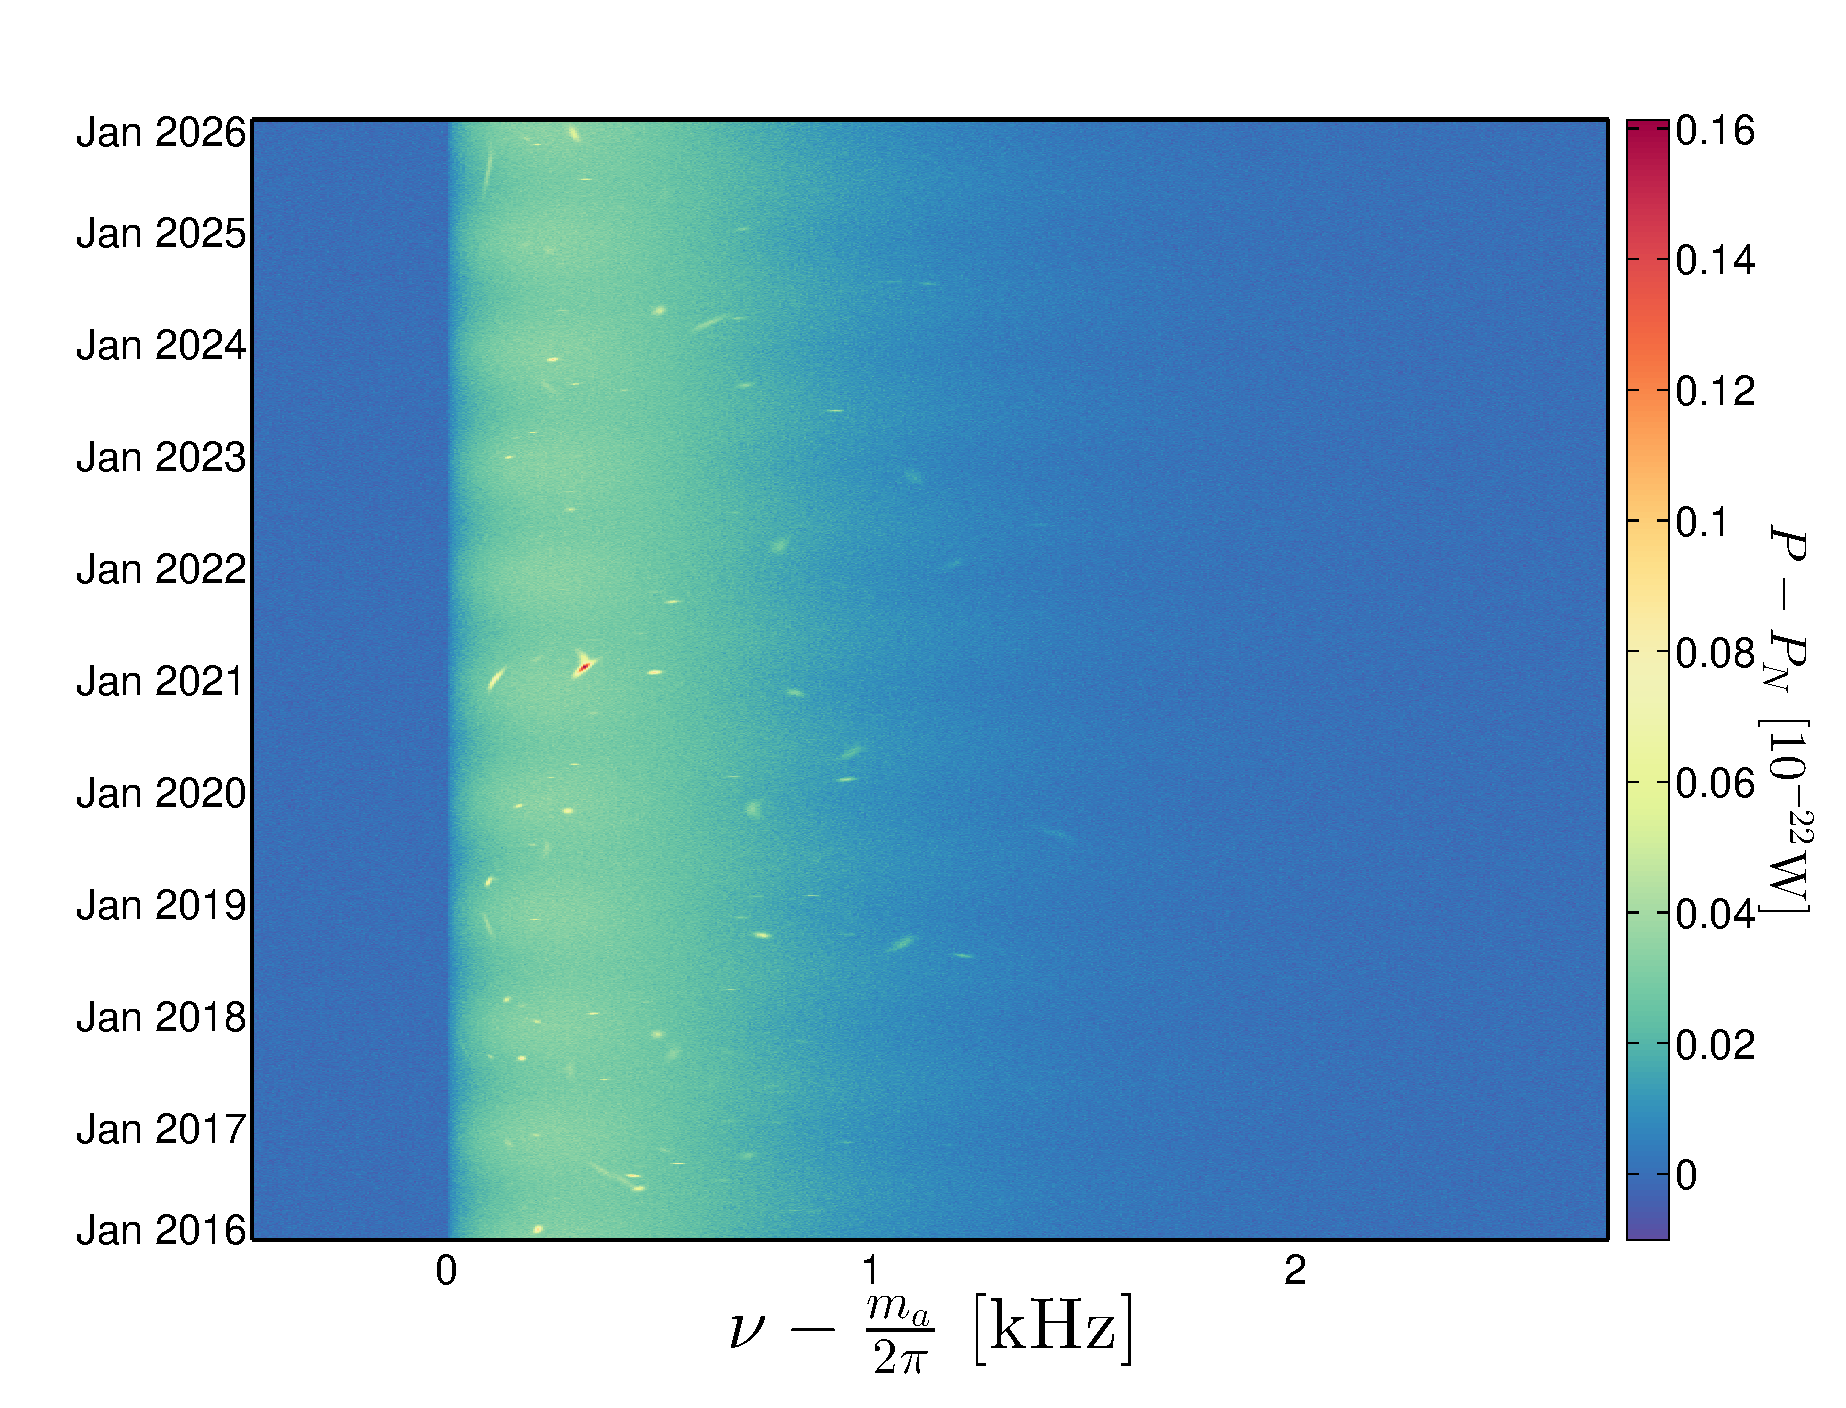
\includegraphics[width=0.8\textwidth]{Figures/miniclusterpowerspectrum.eps}
    \caption[Simulated signal from miniclusters]{Simulated power spectra observed over a 10 year period for a halo model consisting of a smooth population of axion dark matter with an additional component from a network of tidal streams stripped from orbiting miniclusters. The abundance is based on the calculation of Ref.~\cite{Tinyakov:2015cgg}. The signal from minicluster streams appear as short-lived enhancements which are modulated in frequency due to the orbit of the Earth. The power spectra are displayed as a function of time from Jan 2016 to Jan 2021 and frequency shifted by the axion mass.}\label{fig:miniclusterpowerspectrum}
\end{center}
\end{figure}


In Fig.~\ref{fig:miniclusterpowerspectrum} we display a simulated power spectrum observed over a total period of 10 years for a halo consisting of a smooth population of axions and a network of tidal streams from miniclusters. The streams appear as peaks in the power spectrum over a very narrow range of frequencies (as in Sec.~\ref{sec:axions_nbody}) but here since minicluster radii are on the scale of $10^7$~km they are short-lived enhancements compared with usual tidal streams which extend over volumes larger than the scale probed by the Galactic orbit of the Solar System. 

The total power measured in the form of these short-lived enhancements would provide an estimate of the fraction of local axion dark matter contained in minicluster streams from which the abundance of miniclusters could be inferred. We emphasise however that a detailed theoretical treatment of the disruption of a population of miniclusters is still needed in order to fully explore the prospects for their detection. Our example here shows that even if miniclusters comprise only a very small contribution to the local axion density, they appear much more prominently in a high resolution experiment. In principle one could make use of the methods described in Secs.~\ref{sec:axions_reconstruction} and~\ref{sec:axions_nbody} to extract information about individual streams such as their radius, age and Galactic frame velocity as well as place constraints on the minicluster population such as their mass spectrum and abundance, in a complementary way to microlensing, e.g. Ref.~\cite{Fairbairn:2017dmf}. This would require isolating the minicluster signal from both the noise and the background axion power spectrum. A possible strategy could be to use the observations during periods without any minicluster enhancement to make accurate measurements of the underlying parameters (as in Sec.~\ref{sec:axions_reconstruction}) to then subtract the background spectrum thus isolating the stream crossing events. 

A further complication that we have not discussed here is dealing with the presence of any short-lived environmental peaks which may appear in real resonant cavity experiments and could mimic a positive axion signal. These would usually be dealt with by performing a repeat experiment in the frequency range at which the peak was observed. However in the case of minicluster streams which are themselves short-lived this check would not necessarily be successful if the timescales for the environmental peak and the stream crossing were comparable. However a careful treatment of the frequency modulation of the peak over time may in some cases be enough to distinguish a Galactic signal from a lab-based one. We leave a more detailed study of axion minicluster streams and implications for experiments to future work.

\section{Summary}\label{sec:axions_summary}
We have performed a simulation of a hypothetical high resolution ADMX-like experiment following a successful detection of an axion dark matter signal. Our focus here has been on extracting astrophysical information and performing axion astronomy. Our main conclusions are as follows:
\begin{itemize}
\item The measurement of the axion-photon conversion power spectrum enables the accurate reconstruction of both axion particle parameters in conjunction with the underlying astrophysical parameters.
\item With the use of the annual modulation signal one can make accurate measurements of the components of the Solar peculiar velocity. With an experimental duration longer than a year the accuracy can reach below 1~km~s$^{-1}$, which would improve upon the measurement from local astronomical observations.
\item Substructure such as tidal streams appearing in simulations of Milky Way-like halos show up prominently in the resolved axion power spectrum and can hence be measured to levels of sensitivity not possible in the direct detection of WIMPs. The annual modulation signal plays an important role here too as the precise shape of the modulating stream allows the reconstruction of its properties: the Galactic frame velocity, density and dispersion. This in principle would allow axion haloscopes to trace the formation and accretion history of the Milky Way.
\item  We have simulated an approximation to the expected signal from a population of streams from disrupted axion miniclusters. We have extrapolated a result for the calculation of the expected number of stream crossings from Ref.~\cite{Tinyakov:2015cgg}. In an experiment that resolves the axion spectrum the signal from minicluster streams would appear much more prominently in the data and could be isolated to place constraints on their mass spectrum or abundance.
\end{itemize}

The issues we have discussed here are relatively unstudied in the context of axion detection. Hence there are a number of areas in which this study might be extended. We have shown that measuring the axion power spectrum allows accurate reconstruction of underlying parameters and although we have only considered simple models here, in principle the same should be true of other models for the dark matter velocity distribution such as those containing anisotropy parameters or additional substructure such as debris flows~\cite{Kuhlen:2012fz}, dark disks~\cite{Schaller:2016uot} and caustic rings~\cite{Duffy:2008dk}. What remains to be seen however is the extent to which the correct selection of a particular model is possible with data of this kind. This is an important consideration for WIMP direct detection experiments with very low statistics, multiple competing experiments and degeneracy between assumptions about the underlying velocity distribution. These issues have given rise to a number of approaches for making astrophysics independent limits and measurements~\cite{Frandsen:2011gi,Fox:2010bu,Gondolo:2012rs,DelNobile:2013cta,Fox:2014kua,Feldstein:2014gza,Kahlhoefer:2016eds,Gelmini:2016pei} and developing general parameterisations for the velocity distribution~\cite{Peter:2011eu,Kavanagh:2013wba,Kavanagh:2013eya,Kavanagh:2016xfi}. In the case of axions however, because the power spectrum could be measured to an arbitrary level of precision given sufficient duration it may not be necessary to develop any such astrophysics independent methods, however this would require a separate investigation. 

We have used only one axion benchmark mass and coupling, since our focus is on measuring the underlying astrophysical parameters. However our conclusions can be simply extended to other values by considering Eq.~(\ref{eq:totalpower}). Since the total axion power is proportional to $g_{a\gamma\gamma}^2$ one can extend any of the reconstructions to smaller couplings by scaling up the experiment duration, $\tau_{\rm tot}$, by the same factor squared. Although it should be noted that haloscopes can reach smaller couplings by both reducing noise as well as simply extending the duration of the experiment and both of these approaches are necessary for improving constraints on the axion coupling. Since the total power is proportional to $m_a^{-1}$, our conclusions still hold for smaller (larger) values of the axion mass if $\tau_{\rm tot}$ is increased (decreased) by the same factor. The reverse argument goes for values of the local density since the power is linearly proportional to $\rho_a$. However we must take care in extending these results to axion masses much larger or smaller than $\mathcal{O}(\mu$eV) since a given experimental design is only able to probe masses in a small range. There are several reasons for this. First, it is the frequency range of the experiment that dictates the range of axion masses that can be probed. ADMX is suited to masses $<10\, \mu$eV and has currently set constraints between $1.9\,\mu{\rm eV} < m_a < 3.69\,\mu{\rm eV}$~\cite{Asztalos:2009yp,Hoskins:2011iv}. Larger masses require adjustments to the cavity and amplification technology~\cite{Slocum:2014gwa,Baker:2011na}. The Yale Wright Laboratory experiment of Refs.~\cite{Brubaker:2016ktl,Kenany:2016tta} for example operates between 5 - 25 GHz (corresponding to 20 - 100 $\mu$eV) and is the first to set limits for $m_a>20 \mu$eV over a 100 MHz range. 

A number of experimental challenges are present in designing experiments for different mass windows. For higher resonant frequencies the effective volume of the cavity falls off quickly as $\nu^{-3}$ meaning the cavity geometry must be revised to preserve form factors and thus maintain the sensitivity of the experiment. There are also limitations on the frequency ranges for which the SQUID amplification technology is useful meaning new techniques must be developed such as Josephson parametric amplifiers~\cite{Kenany:2016tta} for the GHz range. For masses towards 40~-~400 $\mu$eV the dielectric disk setup of MADMAX~\cite{TheMADMAXWorkingGroup:2016hpc,Millar:2016cjp} has been proposed and avoids the restriction placed on resonators brought about by the dependence on the cavity volume. Smaller masses $10^{-(6-9)}$~eV may also be accessible with nuclear magnetic resonance-based experiments such as CASPEr~\cite{Budker:2013hfa,Graham:2013gfa} or alternative designs with resonant and broadband readout circuits~\cite{Kahn:2016aff}, and LC circuits~\cite{Sikivie:2013laa}.

Ultimately the prospects for axion astronomy will depend on the success of one of the aforementioned search strategies, at which point the development of the optimum technology to measure dark matter axion-photon conversion can begin. In addition to the annual modulation signal, which we have shown to be powerful for making more accurate measurements of some astrophysical parameters, it may also be beneficial to search for possible direction dependent methods (e.g. Refs.~\cite{Irastorza:2012jq,Horns:2012jf,Jaeckel:2015kea}); the angular signature of a dark matter signal encodes much astrophysical information in the context of WIMPs (as we have shown). However in any of these possible scenarios the methods developed in this study will be a valuable step in progressing towards an era of axion astronomy.


